\documentclass[a4paper]{article}
\linespread{1.6}
\usepackage{enumerate}
\usepackage{geometry}
\usepackage{setspace}
\usepackage{amsmath}
\usepackage{amssymb}
\usepackage{cite}
\usepackage[pdftex]{graphicx}
\usepackage{float}
\usepackage{subfigure}
\usepackage{listings}
\geometry{left=1.4cm,right=1.4cm,top=2.5cm,bottom=2.5cm}

\begin{document}
\begin{spacing}{2.0}
\begin{flushleft}\begin{huge}EEL5840 Fundamental Machine Learning   Homework 7\end{huge}\end{flushleft}
\begin{flushright}\begin{Large} Hudanyun Sheng \end{Large}\end{flushright}

\Large{All the code used are attached at the end of this report.}
\normalsize

\section*{\huge\textbf{ Problem \uppercase\expandafter{1} }  }
\normalsize
\noindent
\begin{enumerate}[(1)]
\item When the Fisher discriminant ratio is used as the performance metric for the feature selection method, the related definitions and calculations are listed here:\\
the \textbf{within-class} scatter matrix: $$S_w = \sum_{i=1}^MP_i\Sigma_i$$
where $\Sigma_i = E[(\mathbf{x-\mu_i})(\mathbf{x-\mu_i})^T]$ is the covariance for class $\omega_i$, and $P_i$ is the \textit{a priori} probability of class $\omega_i$.\\
the \textbf{between-class} scatter matrix: $$S_b = \sum_{i=1}^MP_i(\mu_i-\mu_0)(\mu_i-\mu_0)^T$$
where $\mu_0 = \sum_{i=1}^MP_i\mu_i$ is the global mean vector.\\
One definition of the Fisher ratio is: $$J = trace\{S_w^{-1}S_b\}$$
which is that we want to maximize the between class variance and minimize the within class variance at the same time. Diagonal loading is used sometimes to make the matrix $S_b$ is invertible, the fisher ration can also be written as: $$J = trace\{(S_w+\lambda I)^{-1}S_b\}$$
\textbf{Forward feature selection(FFS)} is to sequentially add features, evaluating performance with some performance metric, for here the Fisher ratio, with each potential next feature, adding the feature that improves results.\\
\textbf{Backward feature selection(BFS)} is to sequentially remove features, evaluating performance with the performance metric, removing the feature that does most reduces the performance metric when removed.\\
Based on all discussed above, both forward feature selection and backward selection methods are performed, and their performances are recorded and compared.\\

Some preprocessing procedures are also performed on the data set to compare the result. The method I used to normalize the data is $$\displaystyle\frac{X-X_{min}}{X_{max}-X_{min}}$$

\begin{itemize}
\item \textbf{FFS} 
\begin{enumerate}[(a)]
\item \large{The matrix below shows the ratio of adding every feature \textbf{without} normalization:}
\normalsize

\begin{figure}[H]
\centering
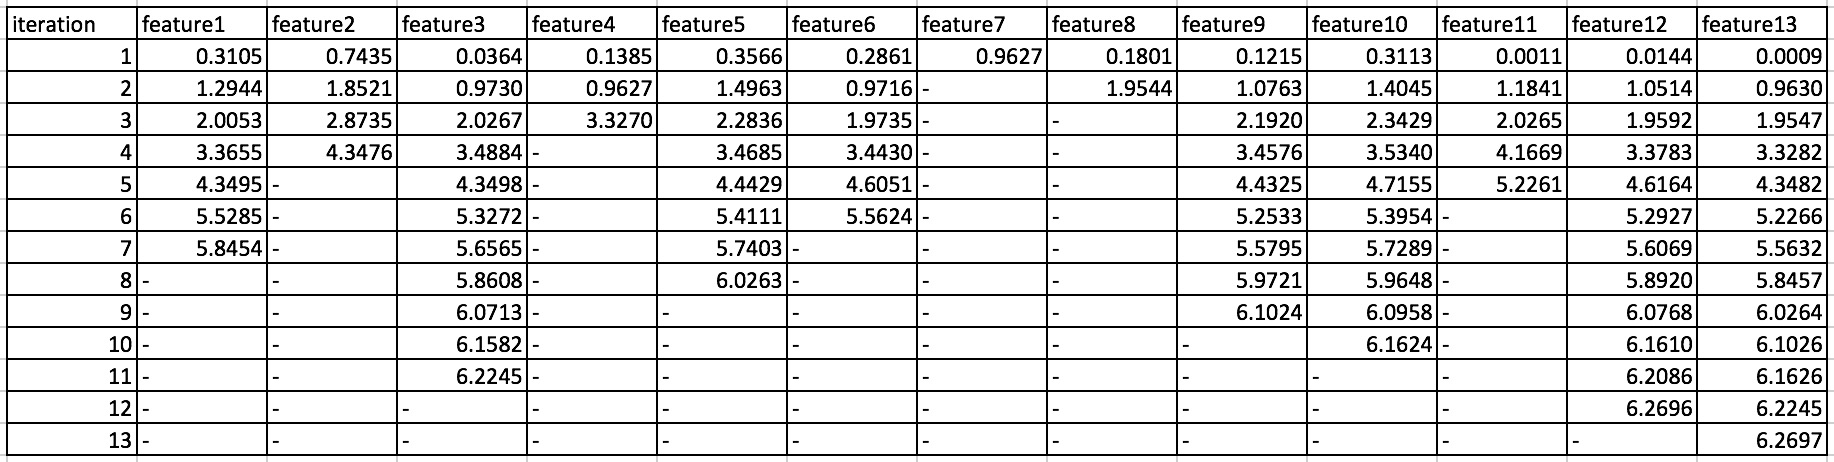
\includegraphics[width = 7.5in]{noNormalizetable.jpg}
%\caption{Table of Fisher ratio changing with every feature added when using Forward feature selection}
\label{FFS}
\end{figure}

The sequence of adding a new feature is 7-8-4-2-11-6-1-5-9-10-3-12-13.
Below is the curve showing how Fisher ratio changes with every new feature added in:
\begin{figure}[H]
\centering
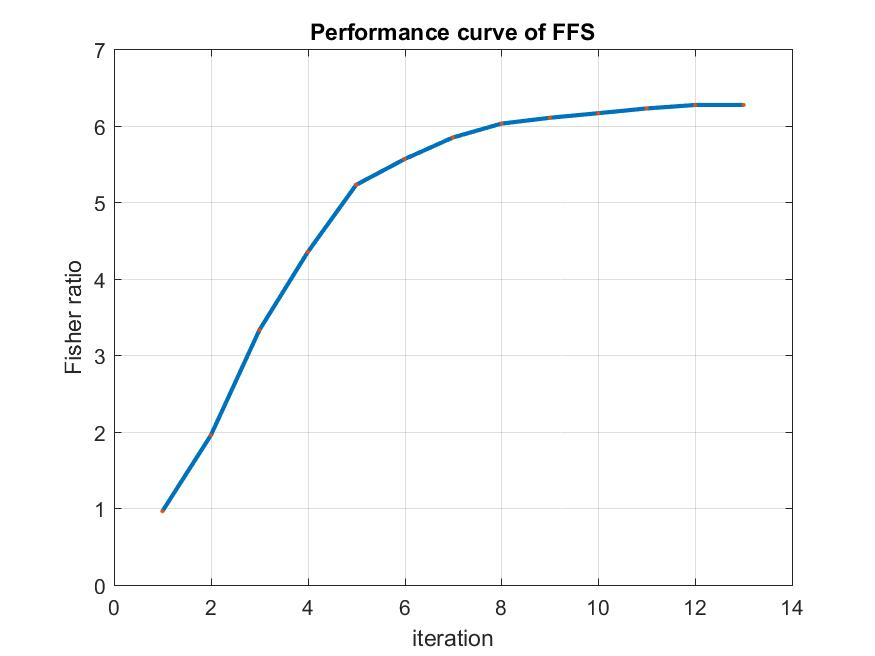
\includegraphics[width = 4in]{FFS.jpg}
\caption{The changing of Fisher ratio with every feature added when using Forward feature selection, without feature normalization}
\end{figure}
We learn from this figure that if we keep adding every another feature, the ratio keep increasing fast until the 8th feature is added in, and the ratio is approaching stable (i.e. not changing any more) after 10-th feature is added in. Both situations would be performed experiment on, i.e. combination of features \{7, 8, 4, 2, 11, 6, 1, 5\} as well as combination of features \{7, 8, 4, 2, 11, 6, 1, 5, 9, 10\} would be tested on. 

\item \large{The matrix below shows the ratio of adding every feature \textbf{with} normalization:}
\normalsize
\begin{figure}[H]
\centering
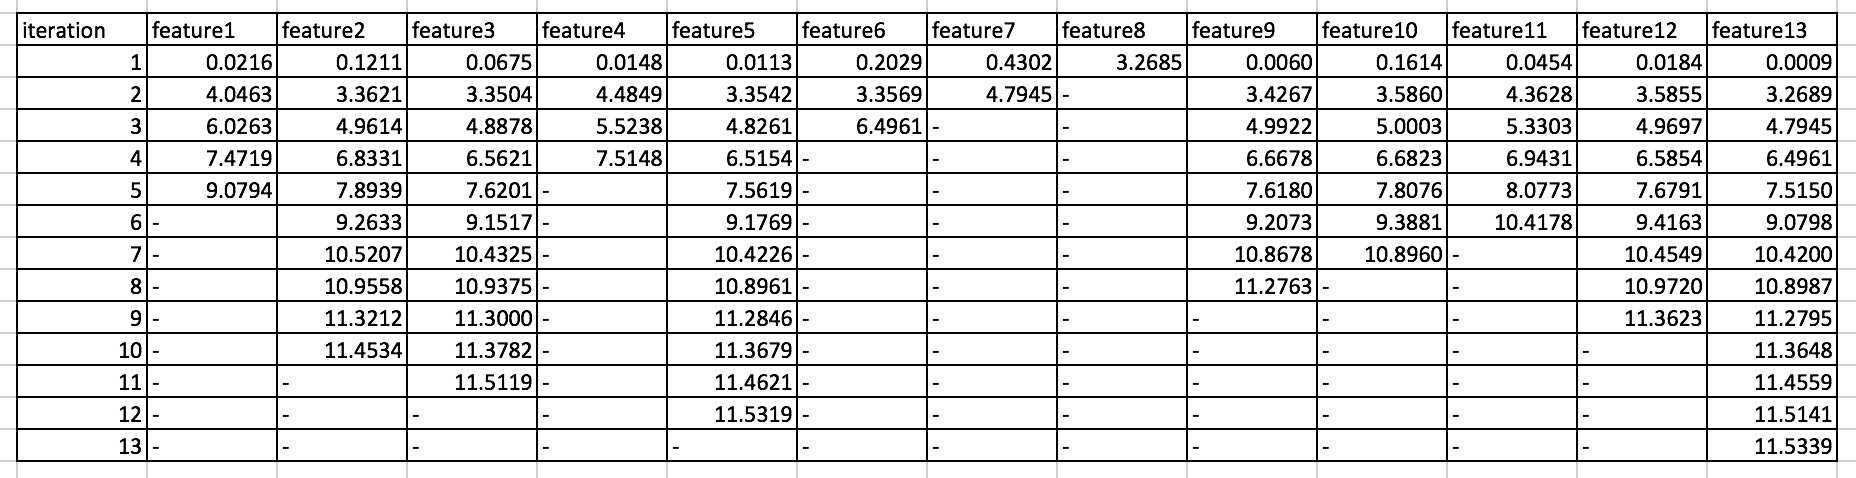
\includegraphics[width = 7.5in]{NormalizetableFFS.jpg}
%\caption{Table of Fisher ratio changing with every feature added when using Forward feature selection, with feature normalization}
\label{FFS}
\end{figure}

The sequence of adding a new feature is 8-7-6-4-1-11-10-9-12-2-3-5-13.
Below is the curve showing how Fisher ratio changes with every new feature added in:
\begin{figure}[H]
\centering
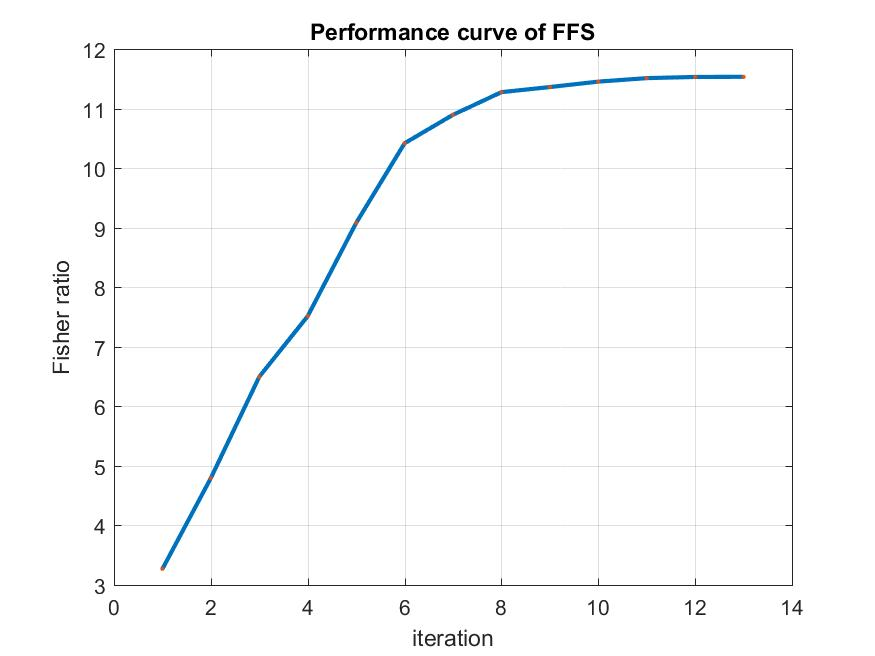
\includegraphics[width = 4in]{FFSnorm.jpg}
\caption{The changing of Fisher ratio with every feature added when using Forward feature selection, with feature normalization}
\end{figure}
We can learn from this figure that if we keep adding every another feature, the ratio keep increasing fast until the 8-th feature is added in, and the ratio is approaching stable (i.e. not changing any more) after 10-th feature is added in. Both situations would be performed experiment on, i.e. combination of features \{8, 7, 6, 4, 1, 11, 10, 9\} as well as combination of features \{8, 7, 6, 4, 1, 11, 10, 9, 12, 2\} would be tested on. 

\end{enumerate}

\item \textbf{BFS}
\begin{enumerate}[(a)]
\item \large{The matrix below shows the ratio of adding every feature \textbf{without} normalization:}
\normalsize
\begin{figure}[H]
\centering
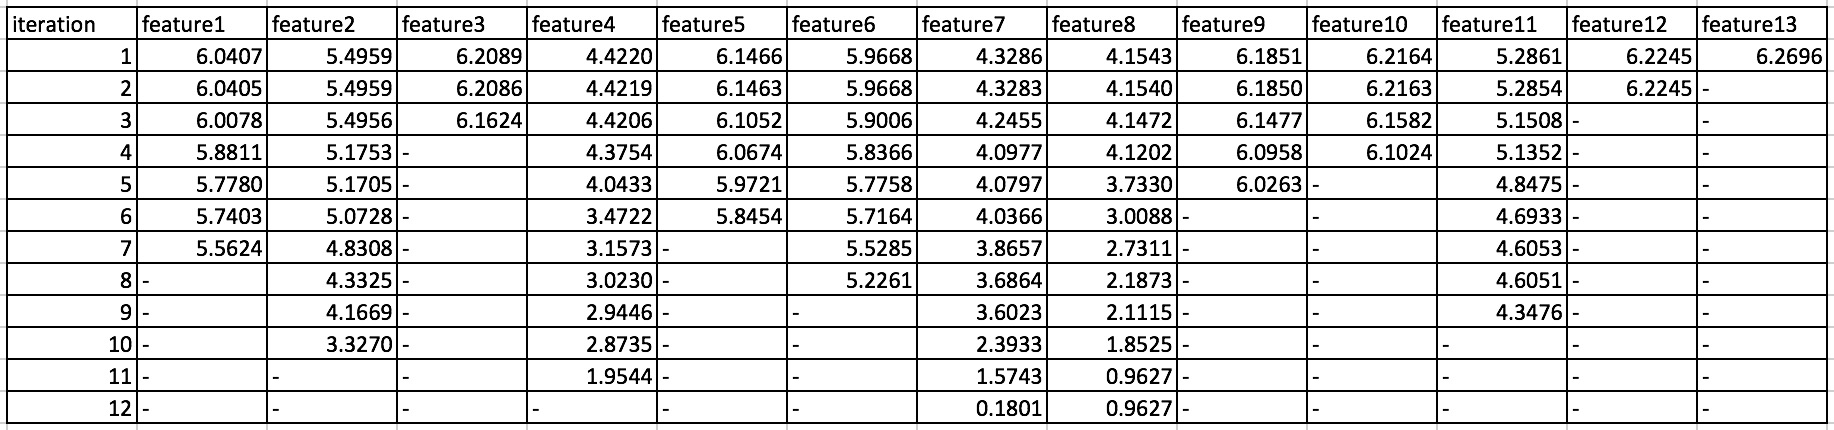
\includegraphics[width = 7.5in]{noNormalizetableBFS.jpg}
%\caption{Table of Fisher ratio changing with every feature added when using Forward feature selection, with feature normalization}
\label{BFS}
\end{figure}

The sequence of dropping another feature is 13-12-3-10-9-5-1-6-11-2-4-8, finally if only one feature is kept, that would be feature 7.
Below is the curve showing how Fisher ratio changes with every new feature dropped from the total feature set:
\begin{figure}[H]
\centering
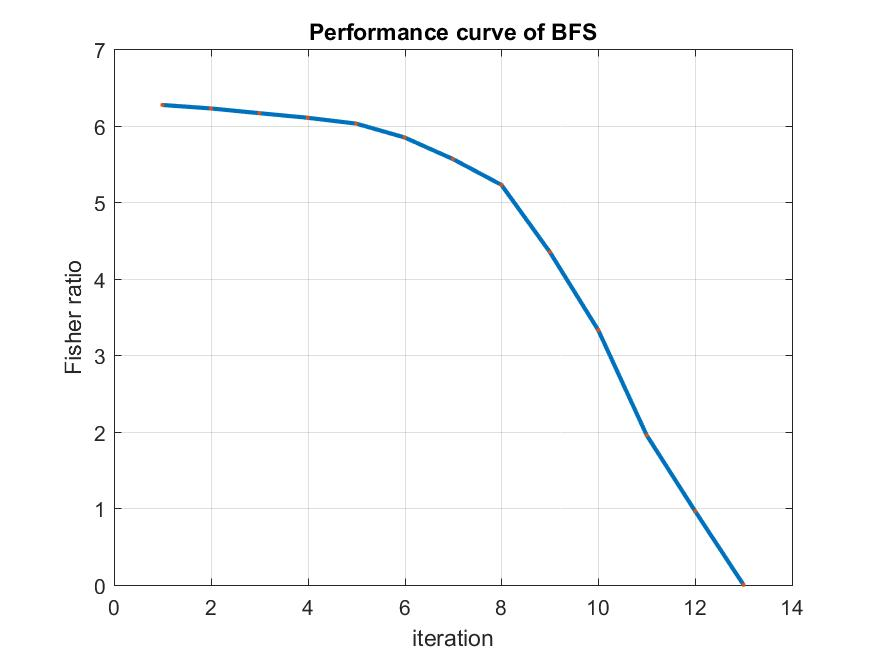
\includegraphics[width = 4in]{BFS.jpg}
\caption{The changing of Fisher ratio with every feature dropped from the total feature set when using Backward feature selection, without feature normalization}
\end{figure}

We can learn from this figure that if we keep dropping every another feature, the ratio keep decreasing slowly (barely not changing) until the 8-th feature is dropped, the ratio starts decreasing quickly. So the result would be features \{6, 11, 2, 4, 8, 7\} should be kept at least, and another test on keeping features \{ 5, 1, 6, 11, 2, 4, 8, 7 \} is also performed.

\item \large{The matrix below shows the ratio of adding every feature \textbf{with} normalization:}
\normalsize
\begin{figure}[H]
\centering
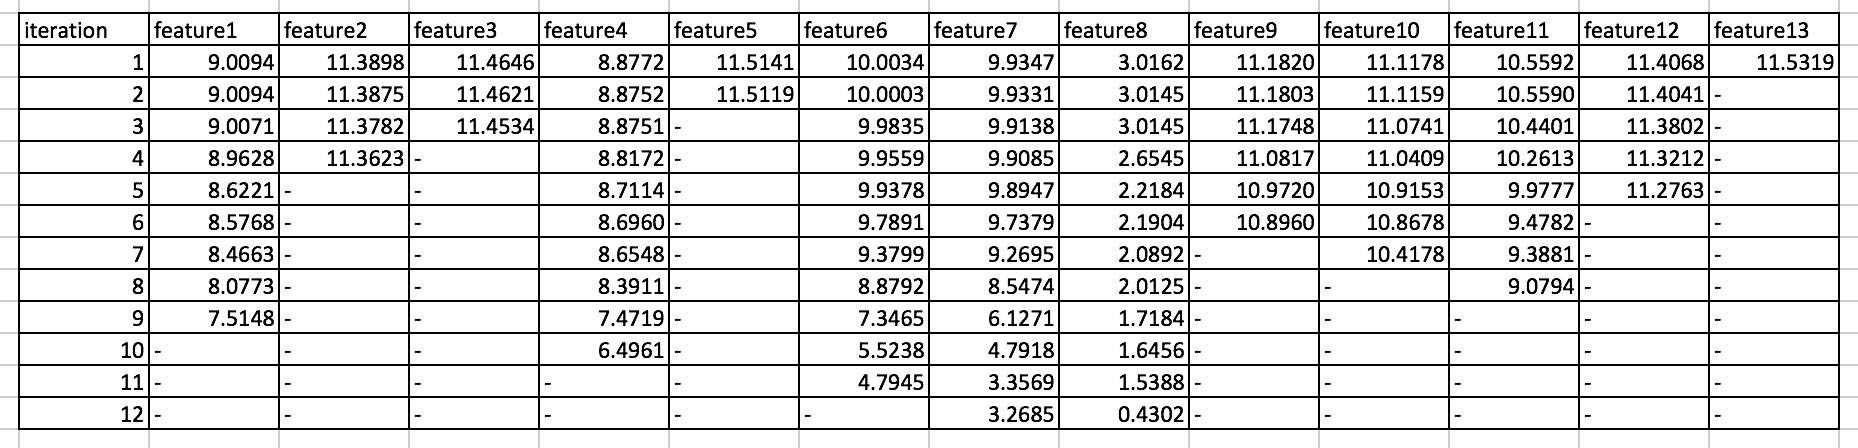
\includegraphics[width = 7.5in]{NormalizetableBFS.jpg}
%\caption{Table of Fisher ratio changing with every feature added when using Forward feature selection, with feature normalization}
\label{BFSnorm}
\end{figure}

The sequence of dropping another feature is 13-5-3-2-12-9-10-11-1-4-6-7-8, if finally only one feature is kept, that would be feature 8.
Below is the curve showing how Fisher ratio changes with every new feature dropped from the total feature set:
\begin{figure}[H]
\centering
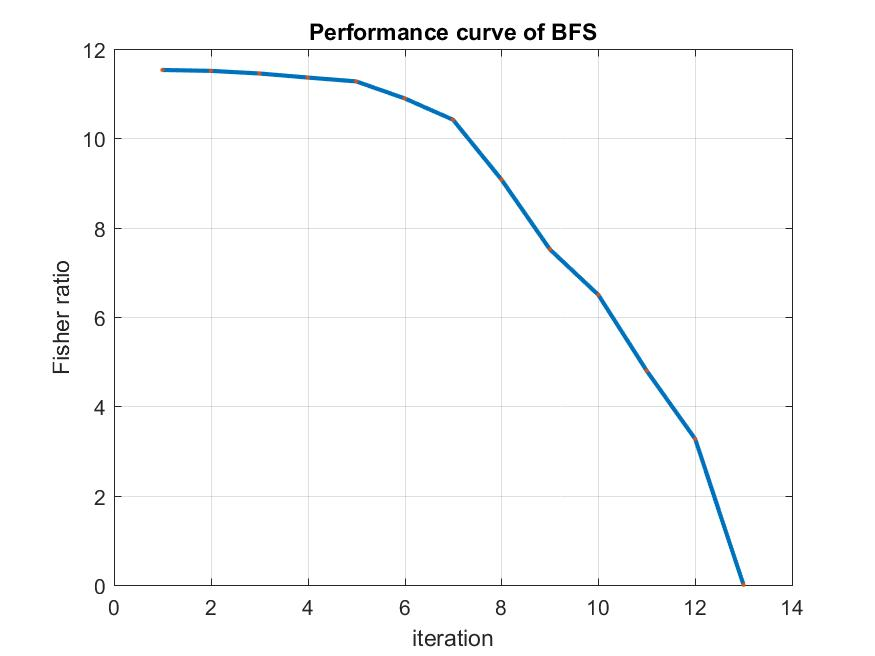
\includegraphics[width = 4in]{BFSnorm.jpg}
\caption{The changing of Fisher ratio with every feature dropped from the total feature set when using Backward feature selection, with feature normalization}
\end{figure}

We can learn from this figure that if we keep dropping every another feature, the ratio keep decreasing slowly (barely not changing) until the 7th feature is dropped, the ratio starts decreasing quickly. So the result would be features \{10, 11, 1, 4, 6, 7, 8\} being kept at least, and another test on keeping features \{ 12, 9,10, 11, 1, 4, 6, 7, 8 \} is also performed.

\end{enumerate}
\end{itemize}

Based on the discussions above, the number of features to be kept are listed in the table below:
\begin{table}[H]
\centering
\begin{tabular}{ccc}
\hline
\ \ & no normalization & with normalization\\
\hline
FFS & 8 & 8\\
BFS & 6 & 6\\
\hline
\end{tabular}
\end{table}

\item Theoretically, I do not think the classification performance using the Bayes Classifier have best performance using the feature set I determined using FFS and BFS. The reasons are listed below:
\begin{itemize}
\item The original data set has the dimension of 13, and with \textbf{forward feature selection} we may finally keep 8 features or so, and with \textbf{backward feature selection} we may finally keep 6 features or so. But no matter the dimension of the data being 13, 8 or 6, the number of the instances is only 6497. Based on \textit{the Curse of dimensionality} the number of the instances is far from enough to densely populate the space of dimension of 6, 8, or 13. 

\item Either \textbf{forward feature selection} or \textbf{backward feature selection} is performed in a greedy way, i.e. the local optima is found every step, but there is no guarantee for global optimal. And this is also the key reason I insist the feature set I determined either using \textbf{FFS} or \textbf{BFS} will not perform better than the full feature set.

\item We choose the features by observing the curve decide when it becomes changing slowly, but actually it is still changing- the Fisher ratio is still increasing after 8-th feature being added in the feature set, and the Fisher ratio is still decreasing after 6-th feature being dropped from the feature set.
\end{itemize}

Experiments are also performed to compare the performance using Bayes Classifier. I use ``0" to represent red wine, and ``1" to represent white wine. $70\%$ of the data are used as training set, the the remaining $30\%$ of the data are used as test set.

First set of experiments compared the performance with or without data normalization. The confusion matrices and the correct classification ratios are calculated. Based on the results I learned the importance of data normalization (though not that obvious in this data set). Later experiments are based normalized data and measured by the correct classification ratio. Later experiments are based normalized data and measured by the correct classification ratio. As stated before, with \textbf{FFS}, 8 features are kept, they are \{ 8, 7, 6, 4, 1, 11, 10, 9\}, and with \textbf{BFS}, 6 features are kept, they are are \{8, 7, 6, 4, 1, 11\}. The table below summaries my results:
\begin{figure}[H]
\centering
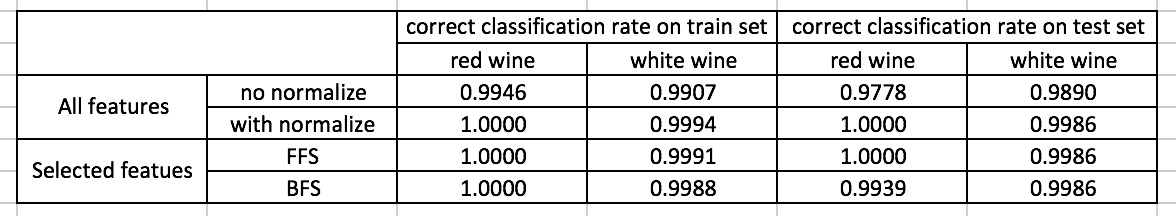
\includegraphics[width = 6in]{allresult.jpg}
\end{figure}
Based on the results above, we would see that the performance with data normalization would be better (though not super obvious in this data set); and on this data set, the performance with feature selected by either FFS or BFS is not better than with full features set. Though conclusions like ``with fewer feature we still get similar results" may be made, but I stick to the comment I made before ``the number of samples is not enough based on the dimension of the given data set for us to make a conclusion". 

\end{enumerate}

\newpage
\section*{\huge\textbf{ Problem \uppercase\expandafter{2} }  }
\normalsize
Below is a summary of how EM learn the parameters:
Initialize mixture component mean $\mu_i$, variance $\Sigma_i$, and proportion $\pi_i$.\\
The ``responsibility" of every component for every data point is calculated $C_{ik} = p(z_i = k|x_i, \theta) = \displaystyle\frac{\pi_i^tp_{z_i}(x_i|\theta_{z_i}^t, z_i)}{\sum_{k=1}^K\pi_i^tp_{z_i}(x_i|\theta_{z_i}^t, z_i)}$. 
Then $\mu$, $\Sigma$, and $\pi$ are updated iteratively. 
\noindent
\begin{enumerate}[(1)]
\item Since the \textbf{EM algorithm} need the input of the number of mixture component, before EM is implemented to determine the mixture proportion, PCA is performed to get some initial guess of number of mixture components. The original dimension of the data set is 5, so I tried to project it into dimension of 3. The visualizations are shown below:
\begin{figure}[H]
\centering
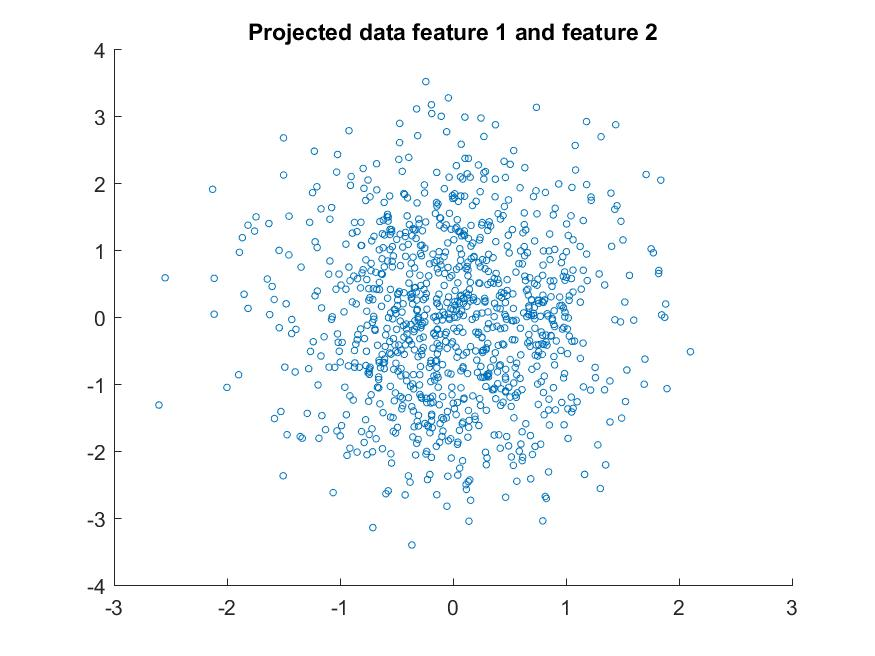
\includegraphics[width = 1.5in]{p1and2.jpg}
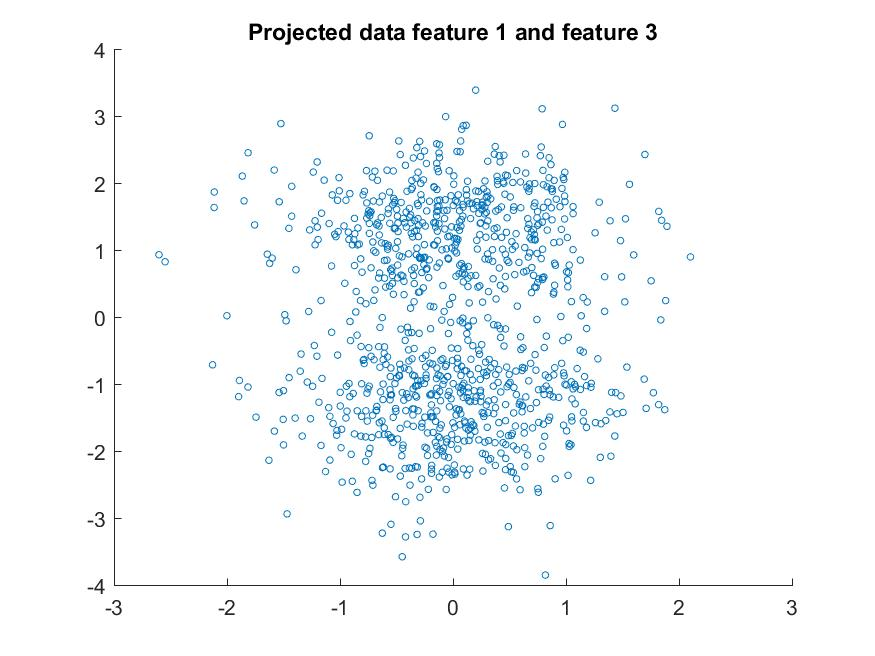
\includegraphics[width = 1.5in]{p1and3.jpg}
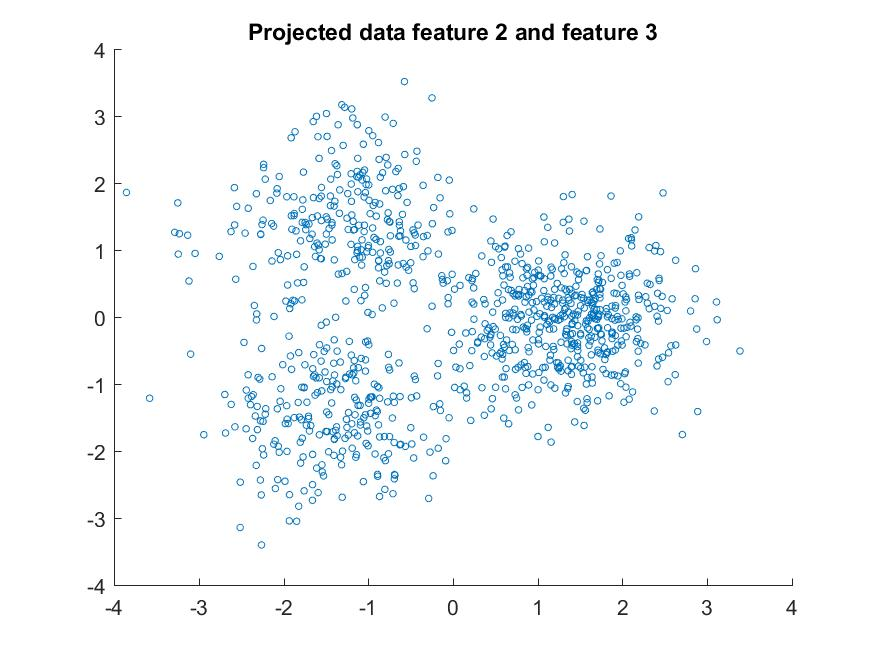
\includegraphics[width = 1.5in]{p2and3.jpg}
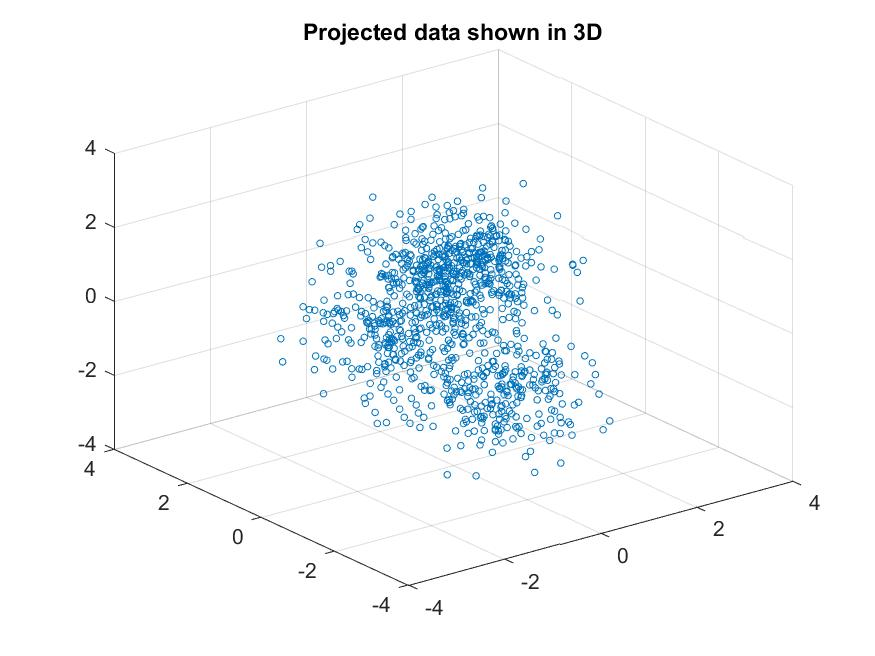
\includegraphics[width = 1.5in]{p3d.jpg}
\caption{From left to right: the scatter plot with feature 1 and 2 after performing PCA, the scatter plot with feature 1 and 3 after performing PCA, the scatter plot with feature 2 and 3 after performing PCA, the 3D scatter plot with all 3 features after performing PCA.}
\end{figure}
%\begin{figure}[H]
%\centering
%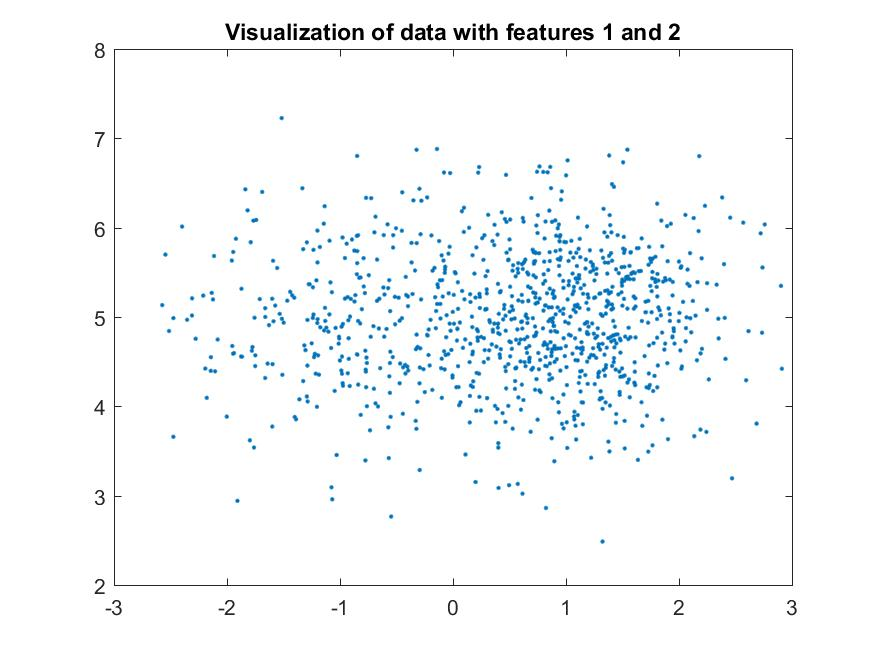
\includegraphics[width = 3in]{V1and2.jpg}
%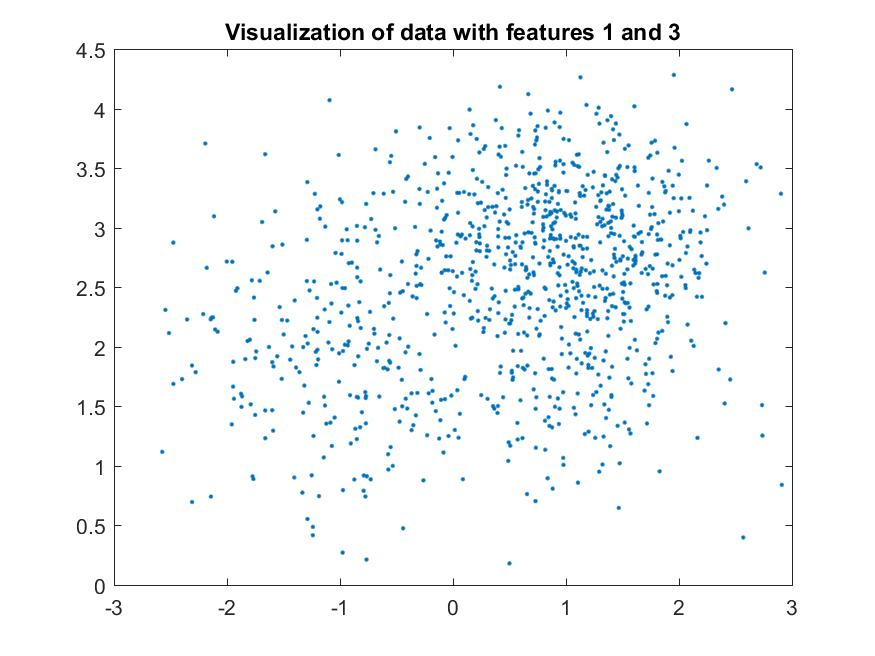
\includegraphics[width = 3in]{V1and3.jpg}
%\end{figure}
%\begin{figure}[H]
%\centering
%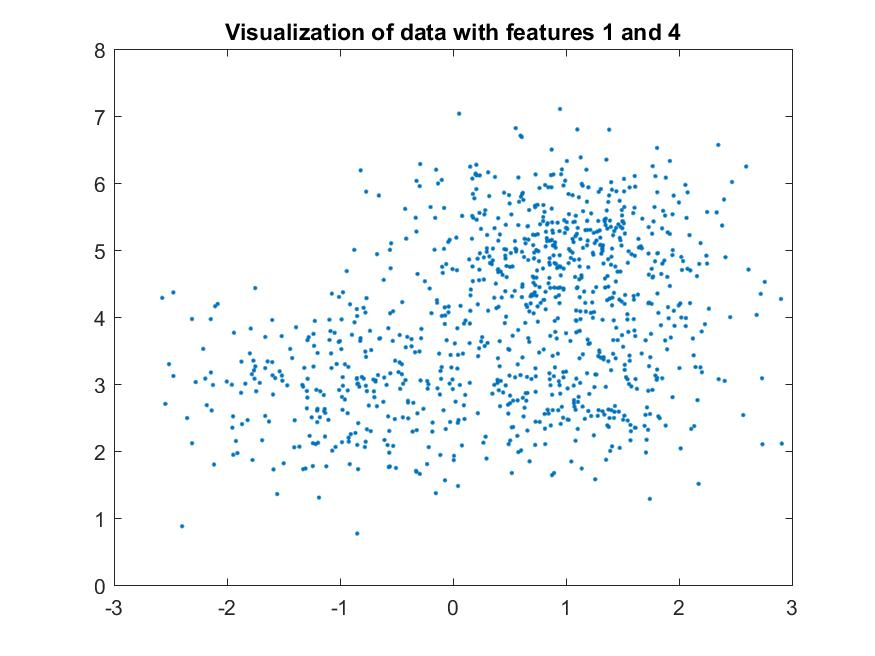
\includegraphics[width = 3in]{V1and4.jpg}
%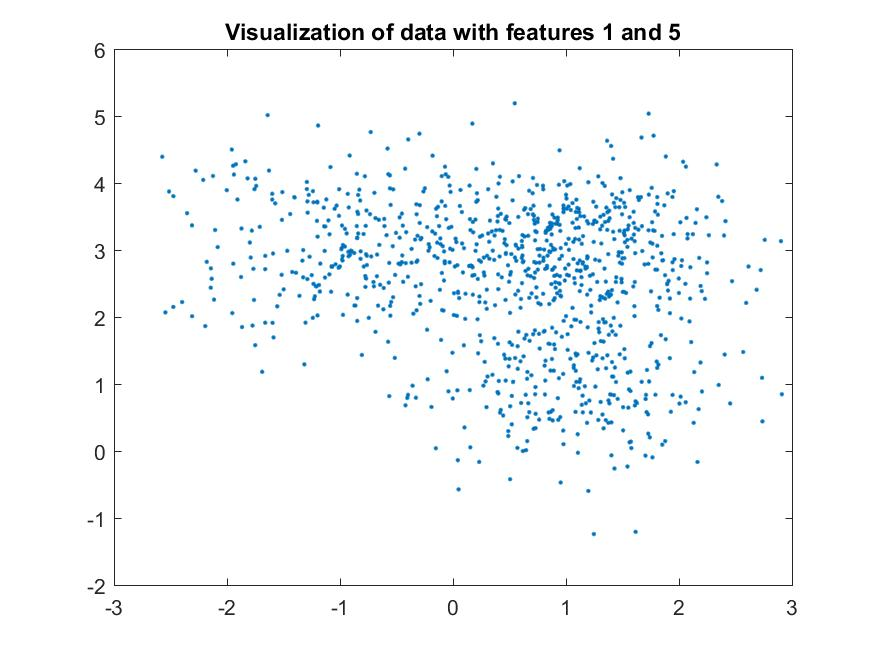
\includegraphics[width = 3in]{V1and5.jpg}
%\end{figure}
%\begin{figure}[H]
%\centering
%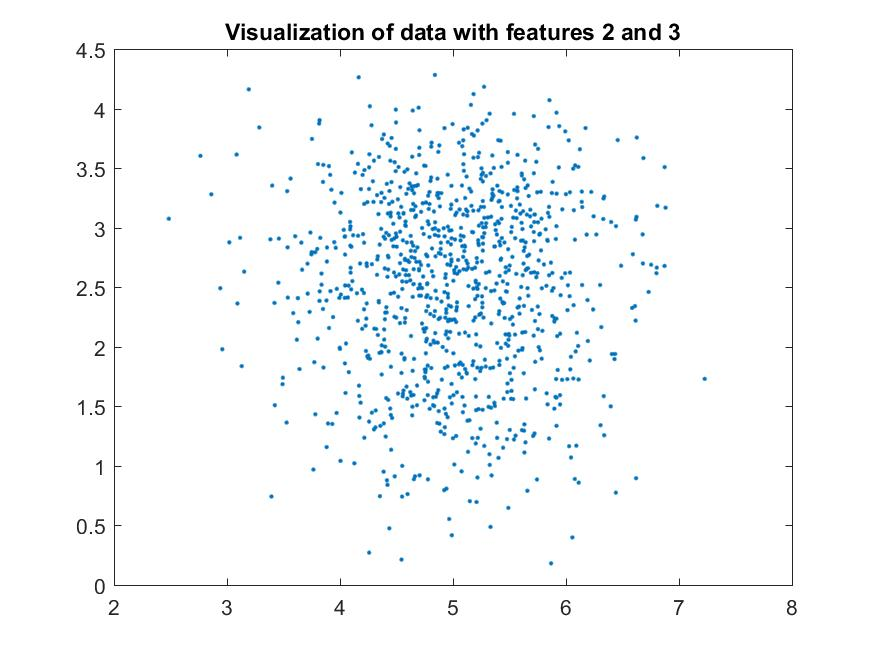
\includegraphics[width = 3in]{V2and3.jpg}
%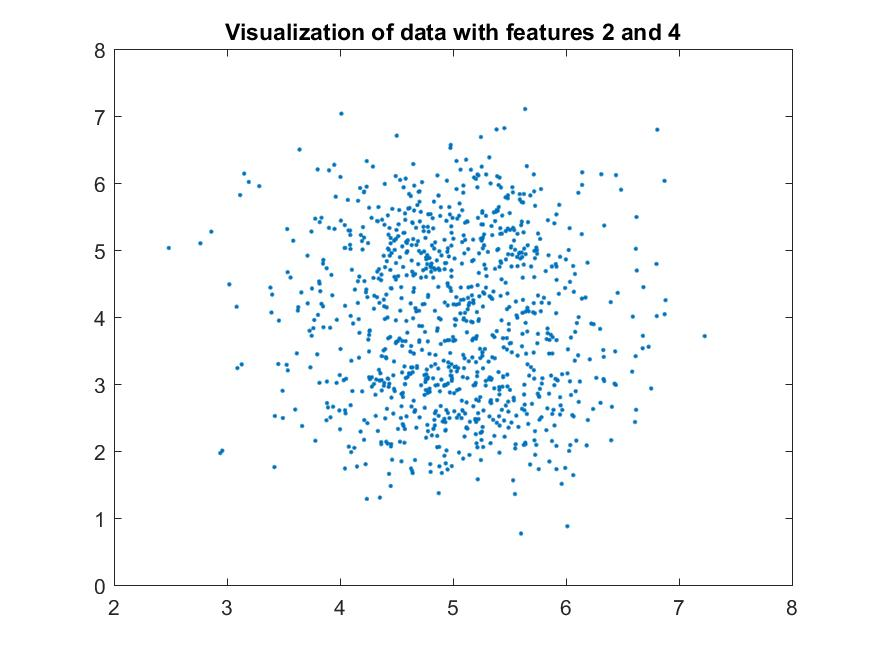
\includegraphics[width = 3in]{V2and4.jpg}
%\end{figure}
%\begin{figure}[H]
%\centering
%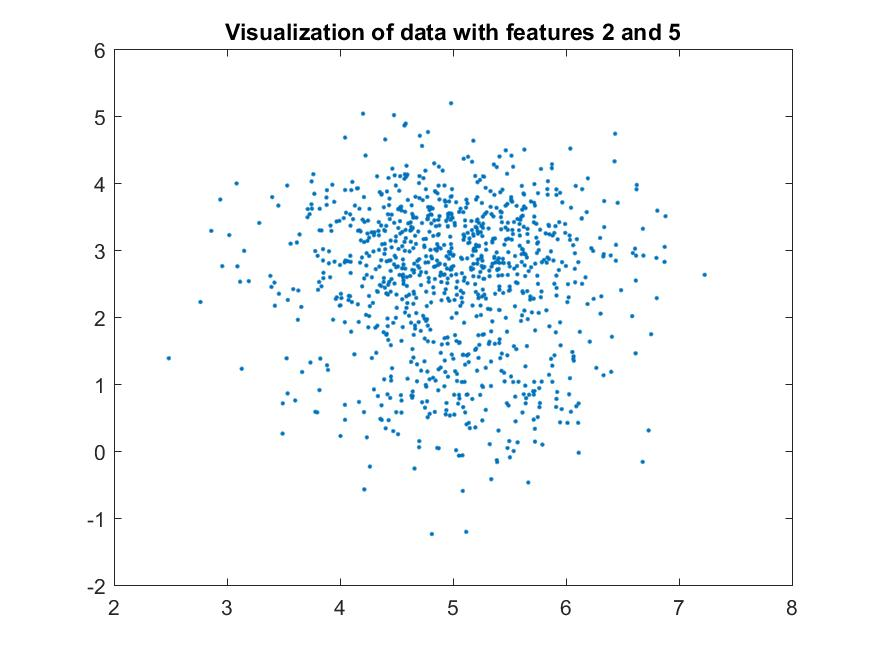
\includegraphics[width = 3in]{V2and5.jpg}
%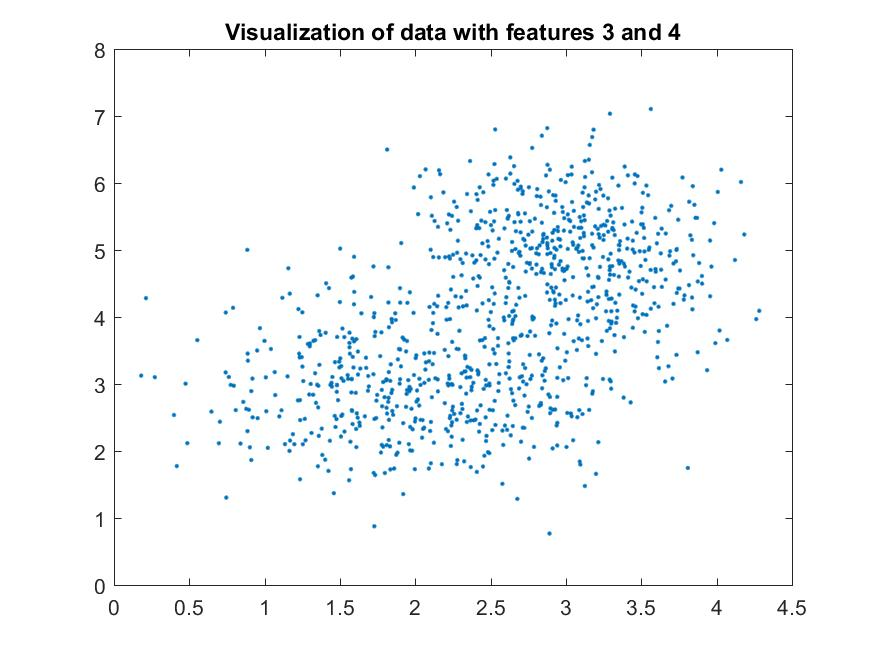
\includegraphics[width = 3in]{V3and4.jpg}
%\end{figure}
%\begin{figure}[H]
%\centering
%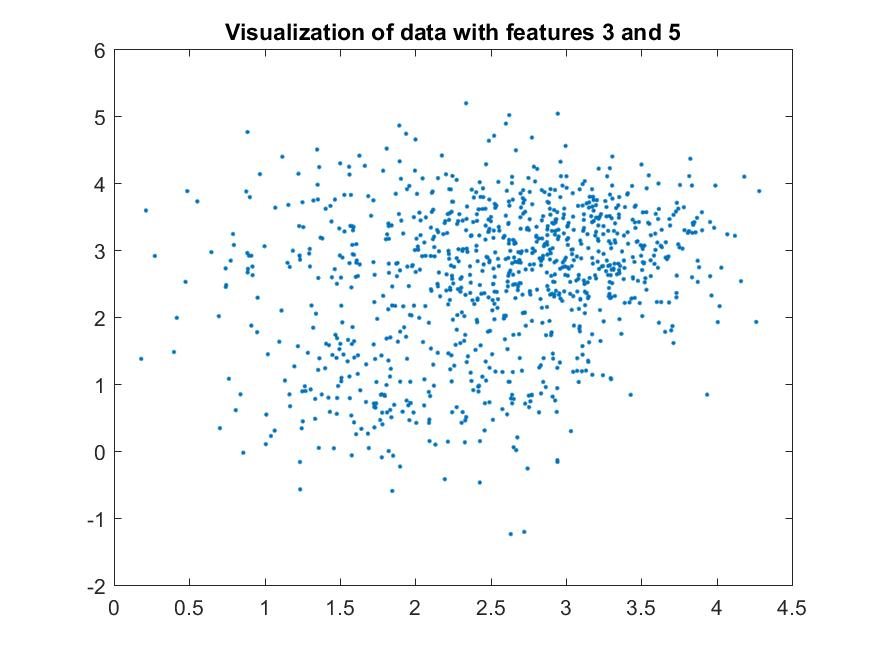
\includegraphics[width = 3in]{V3and5.jpg}
%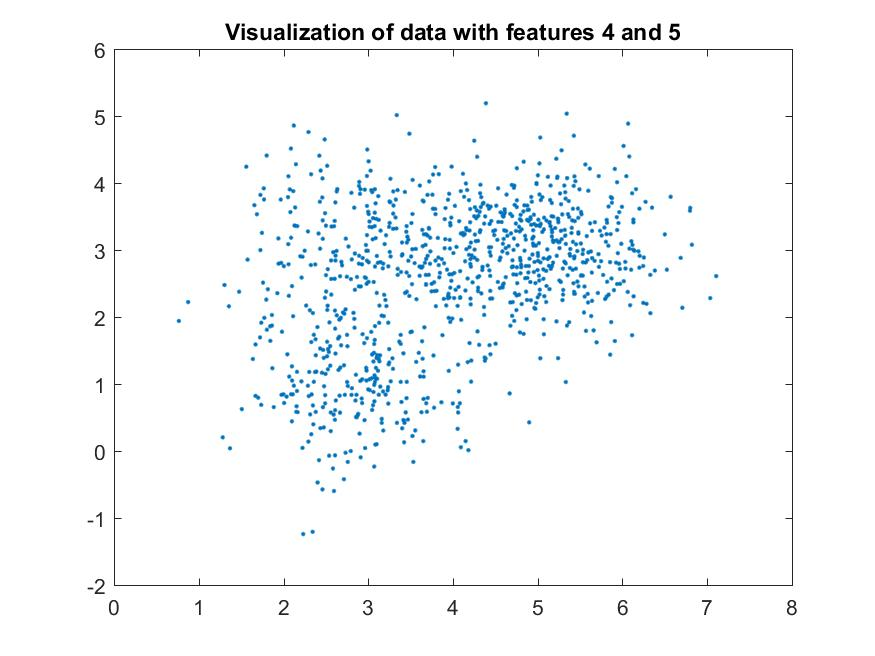
\includegraphics[width = 3in]{V4and5.jpg}
%\end{figure}
With the help of principal component analysis and the visualization, I go the initial guess of the number of mixture components may be 3. It can also be greater than 3.\\
Then \textbf{EM algorithm} is implemented on the data set. I started with setting the ``number of mixture components" to 3. The result of EM is shown below. In this figure, the colors are considered as ``pseudo color", i.e. for a given data point, different ``responsibilities" of different mixture component would result in different color.
\begin{figure}[H]
\centering
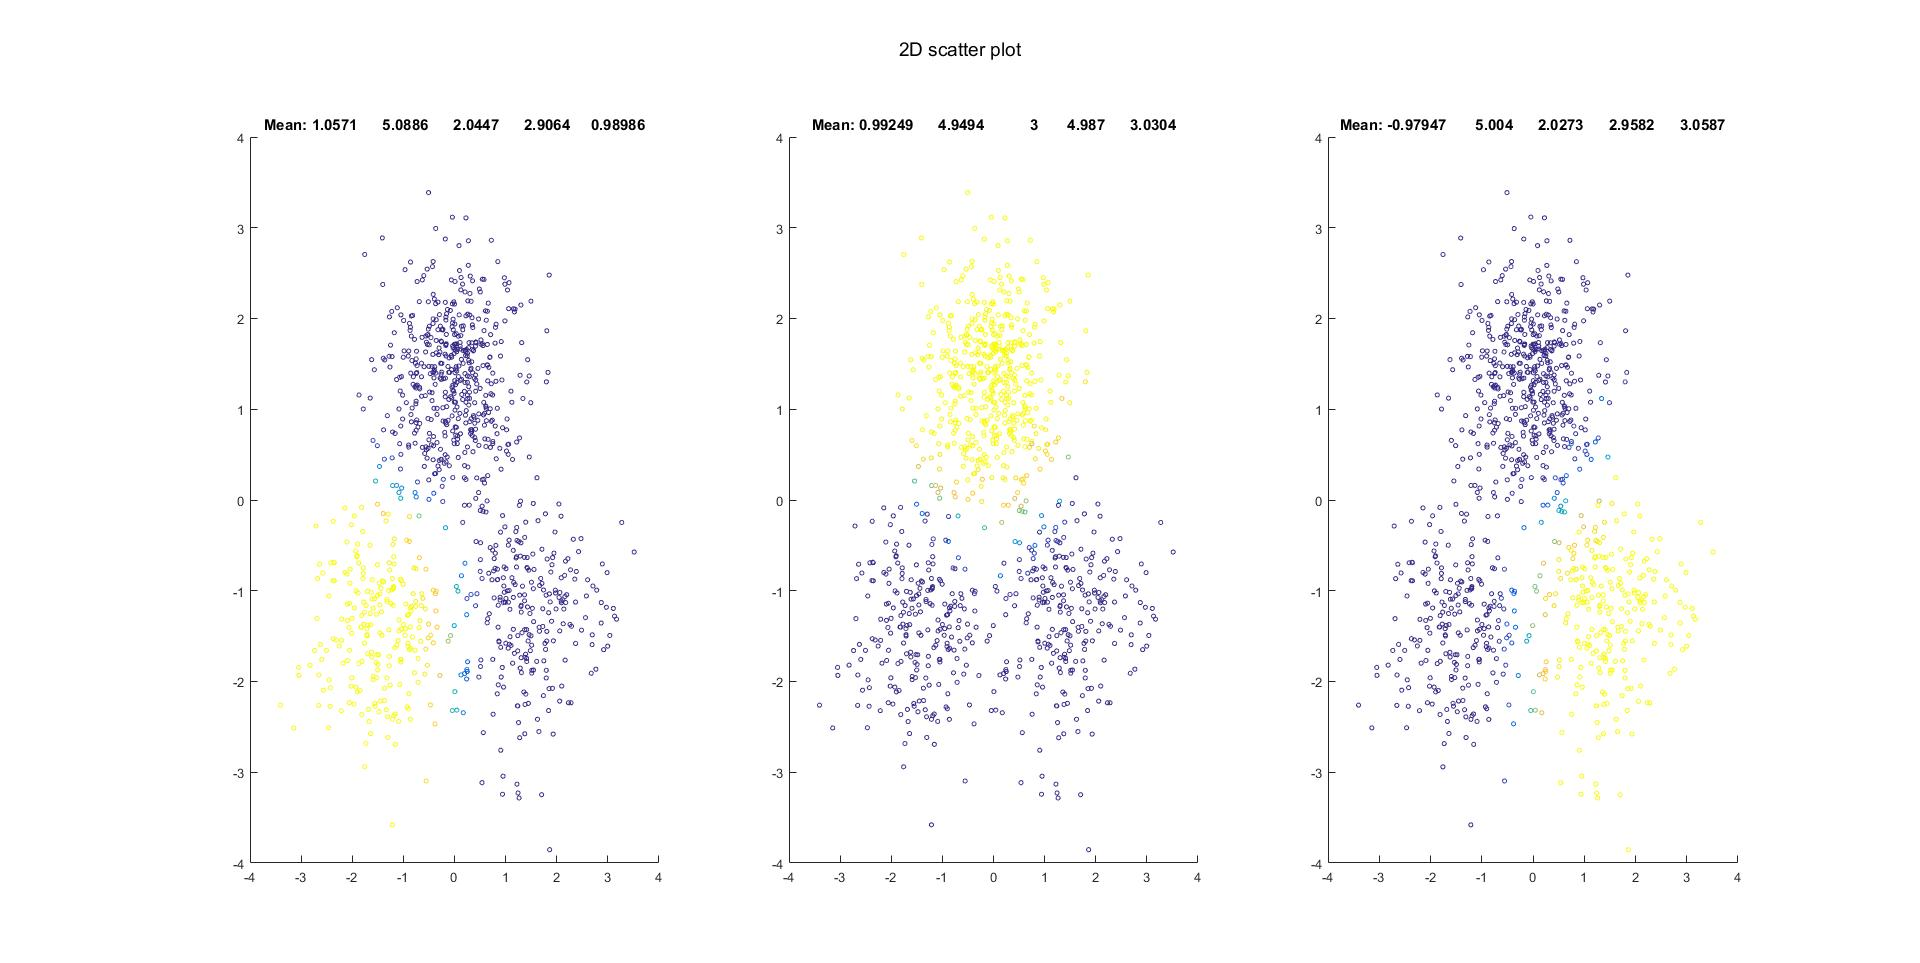
\includegraphics[width = 6in]{scatter2d.jpg}
\end{figure}

\begin{figure}[H]
\centering
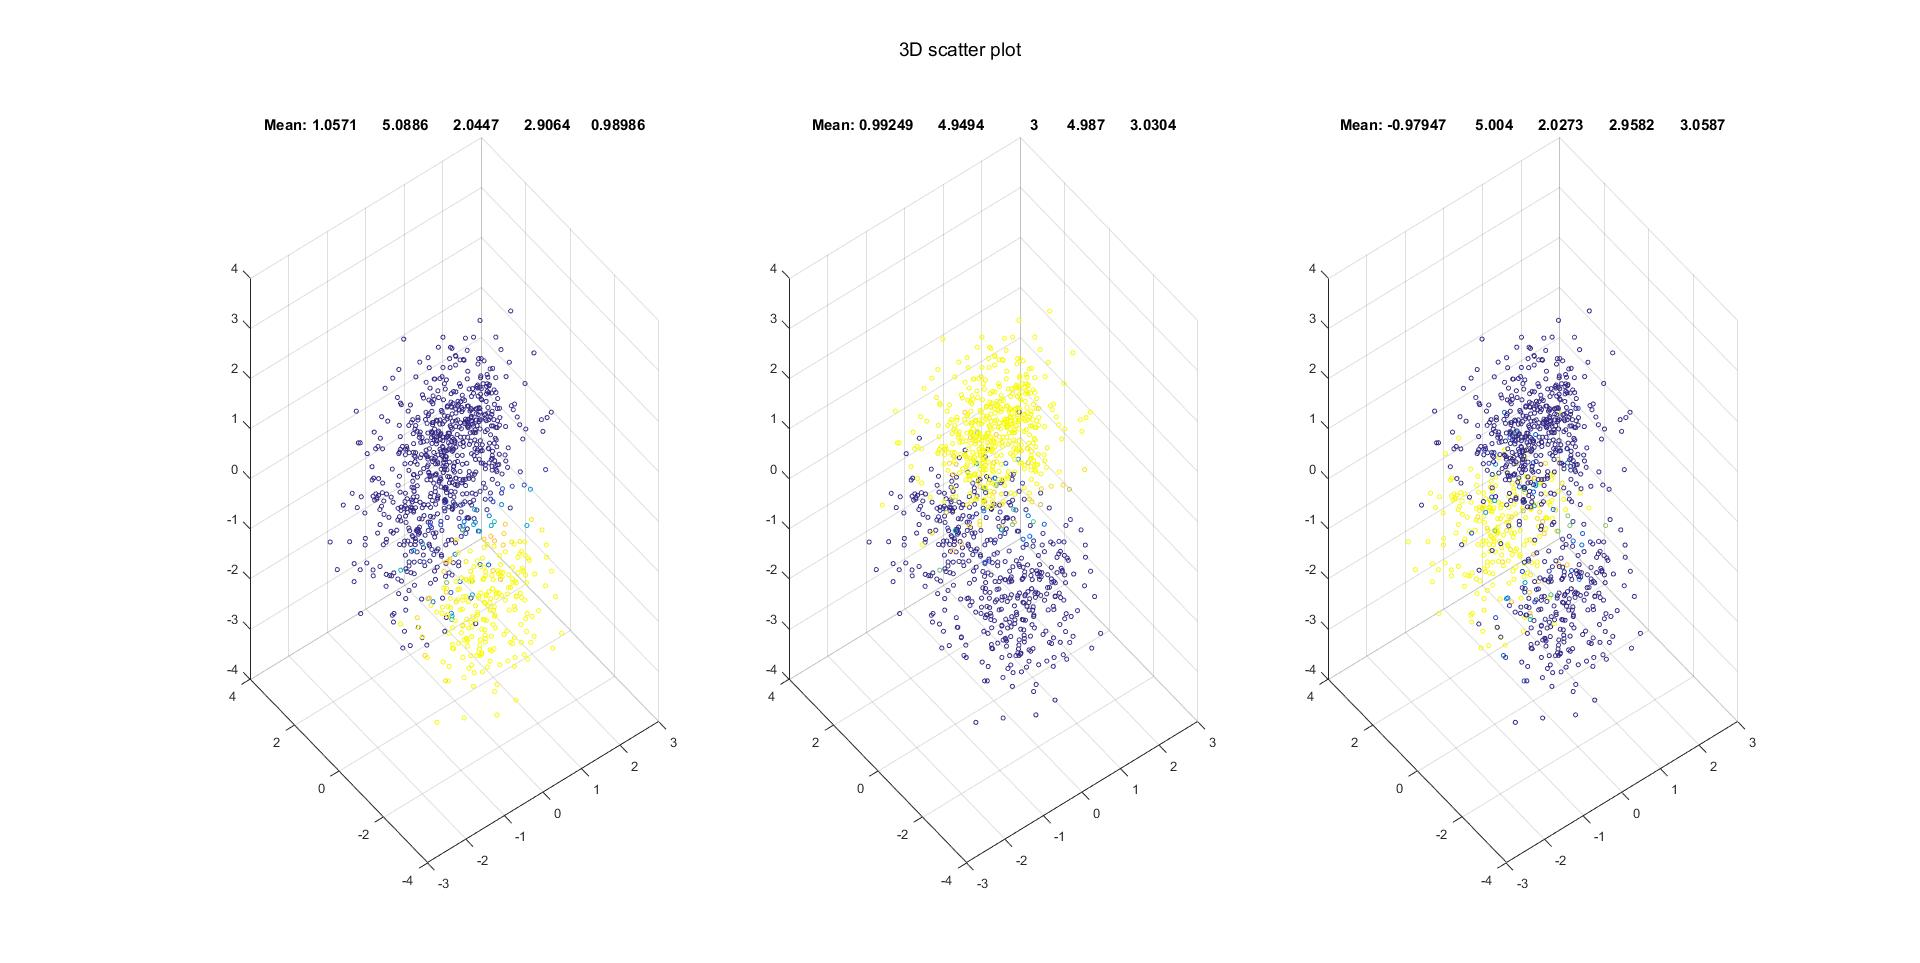
\includegraphics[width = 6in]{scatter3d.jpg}
\end{figure}

The results of experiments I did are shown below, the parameters  learned are pretty consistent:
\begin{figure}[H]
\centering
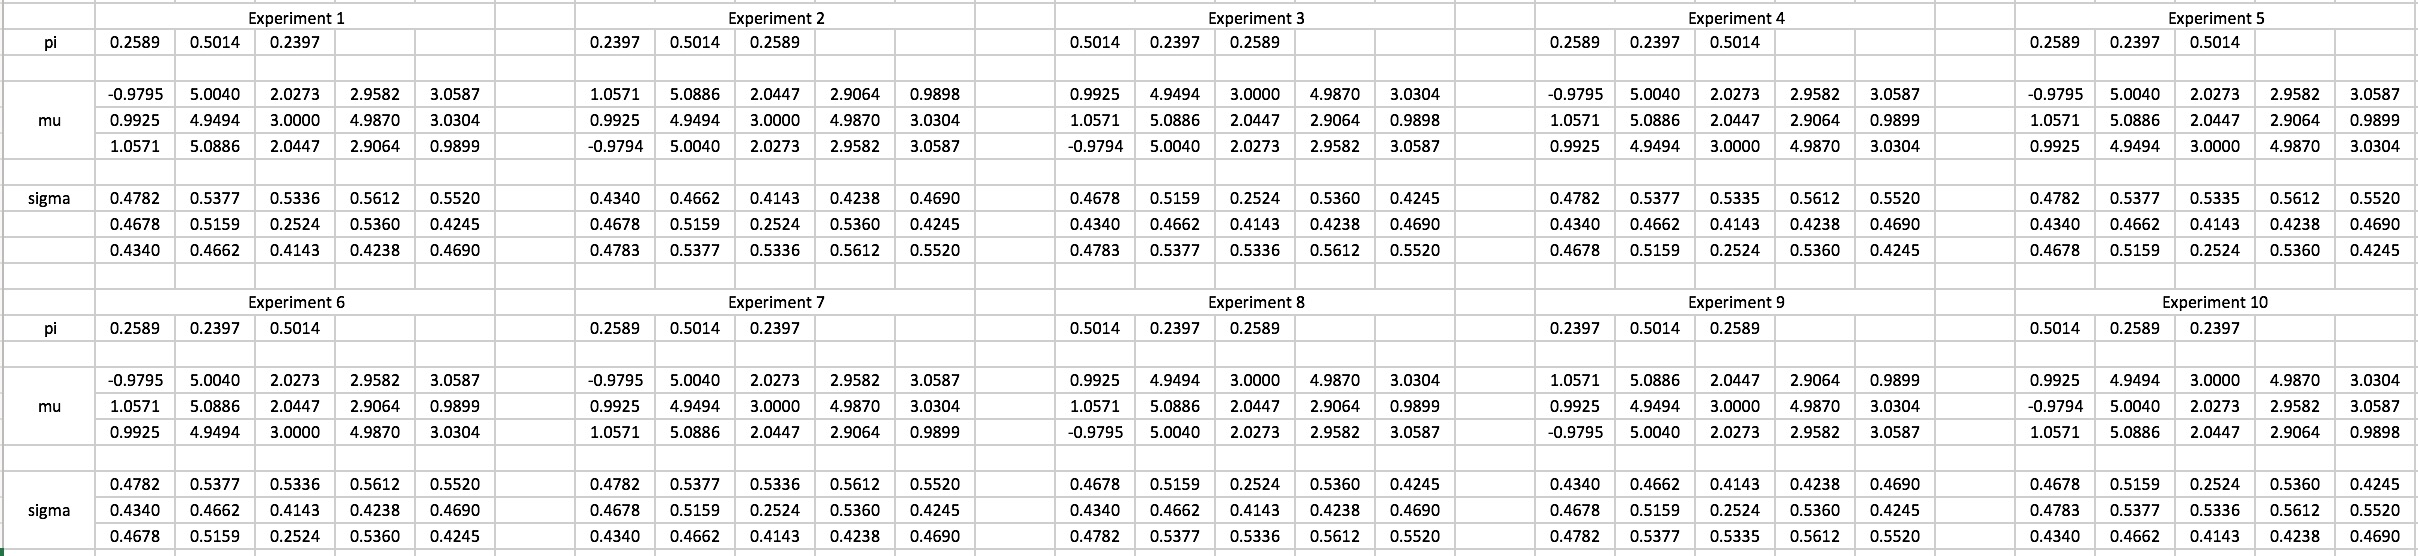
\includegraphics[width = 7in]{EM3.jpg}
\end{figure}

From the figures above, I concluded that if assuming 3 mixture components, the clusters are pretty consistent. And also, by performing the EM algorithm several times, the mixture proportions as well as the mean and covariance for every cluster are also pretty consistent.\\
If assuming 4 mixture components, the mixture proportions as well as the mean and covariance for every cluster are not consistent. The results of experiments I did are shown below, the parameters  learned are not consistent:
\begin{figure}[H]
\centering
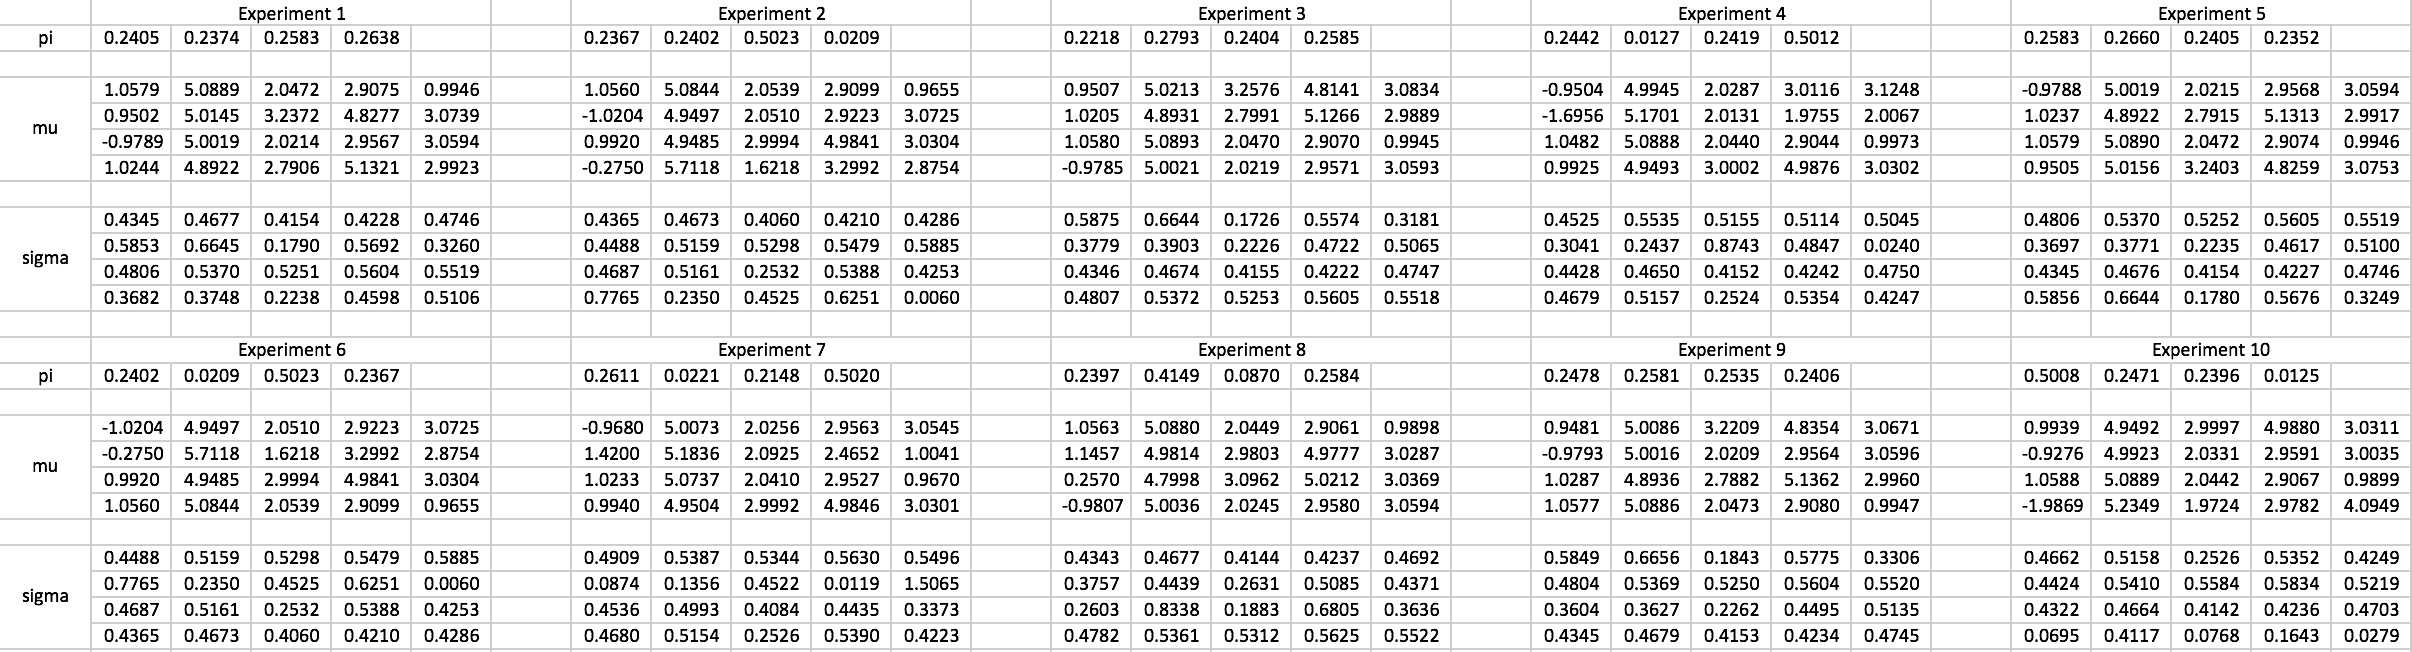
\includegraphics[width = 7in]{EM4.jpg}
\end{figure}

One of the scatter plots are shown below:
\begin{figure}[H]
\centering
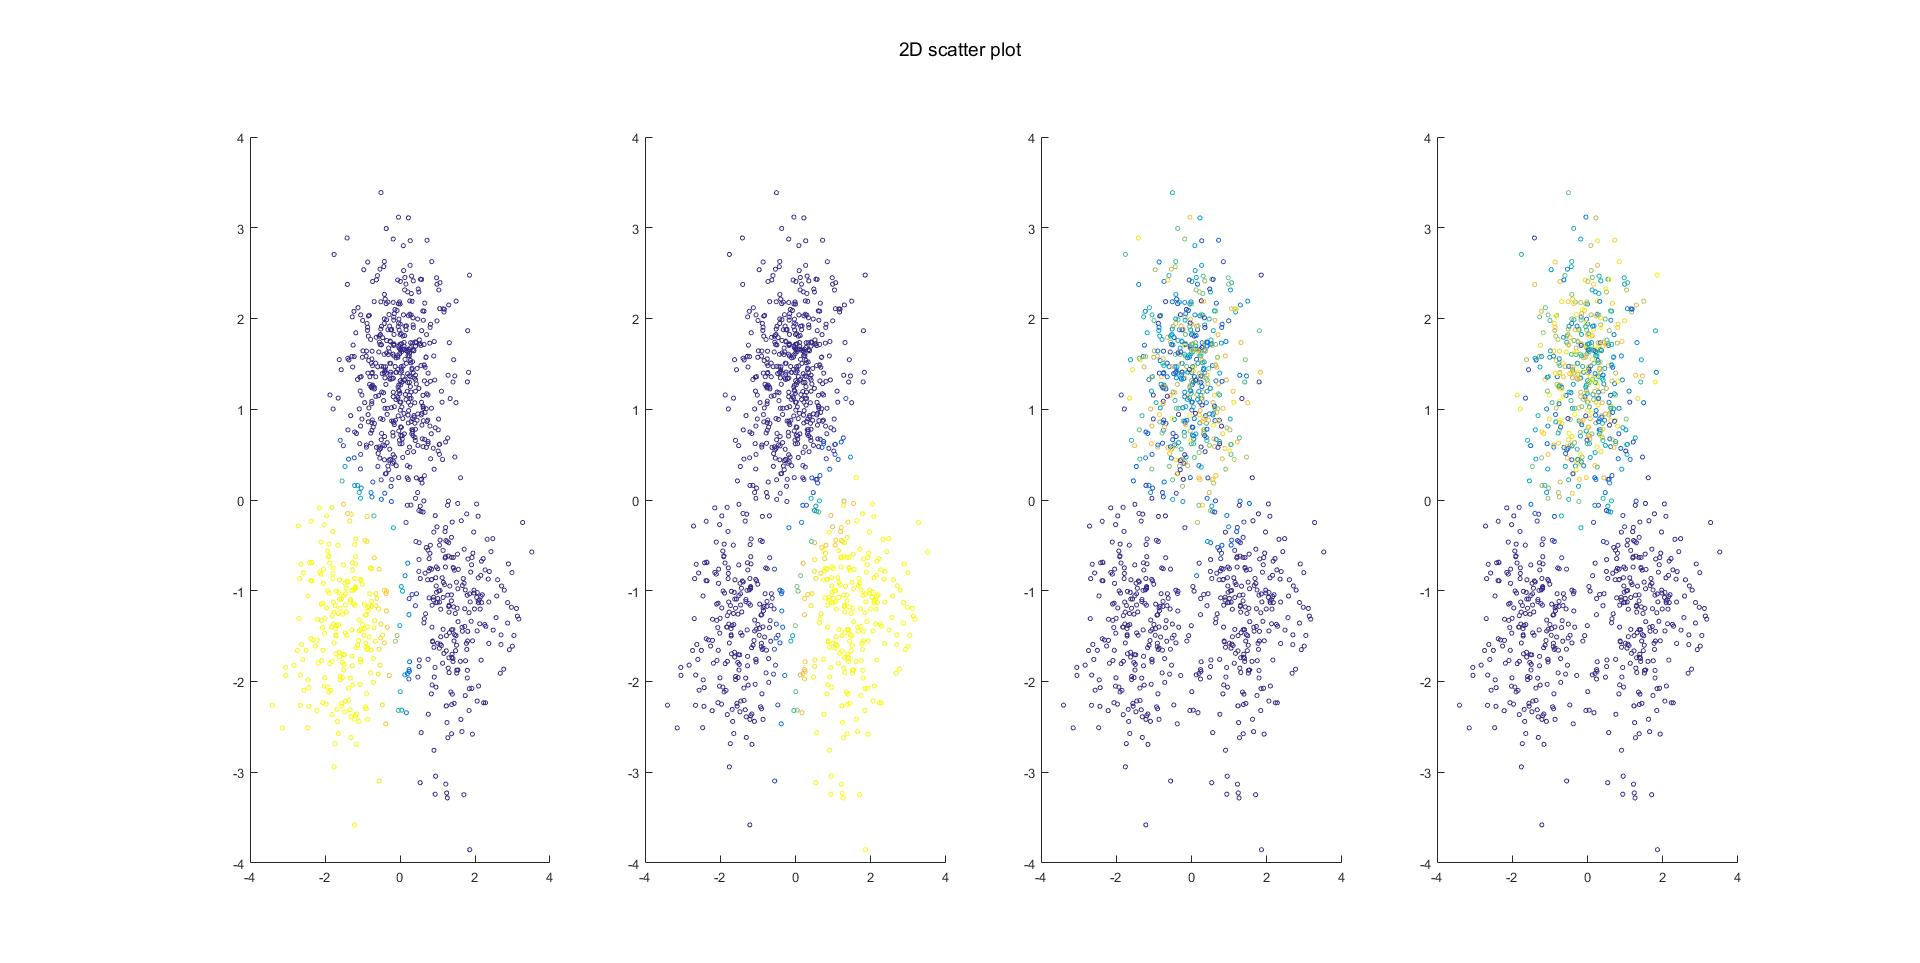
\includegraphics[width = 6in]{scatter2d4.jpg}
\caption{2-d scatter plot assuming 4 component}
\end{figure}
From the figures we can also see that there are two clusters which are pretty consistent, but the other two are always mixing together. And also from the experiment results, by run the EM code several, the parameters changed a lot and are not consistent. Sometimes the mixture proportion for one cluster is tend to be really small, which is a sign to merge with other cluster(s).
\begin{figure}[H]
\centering
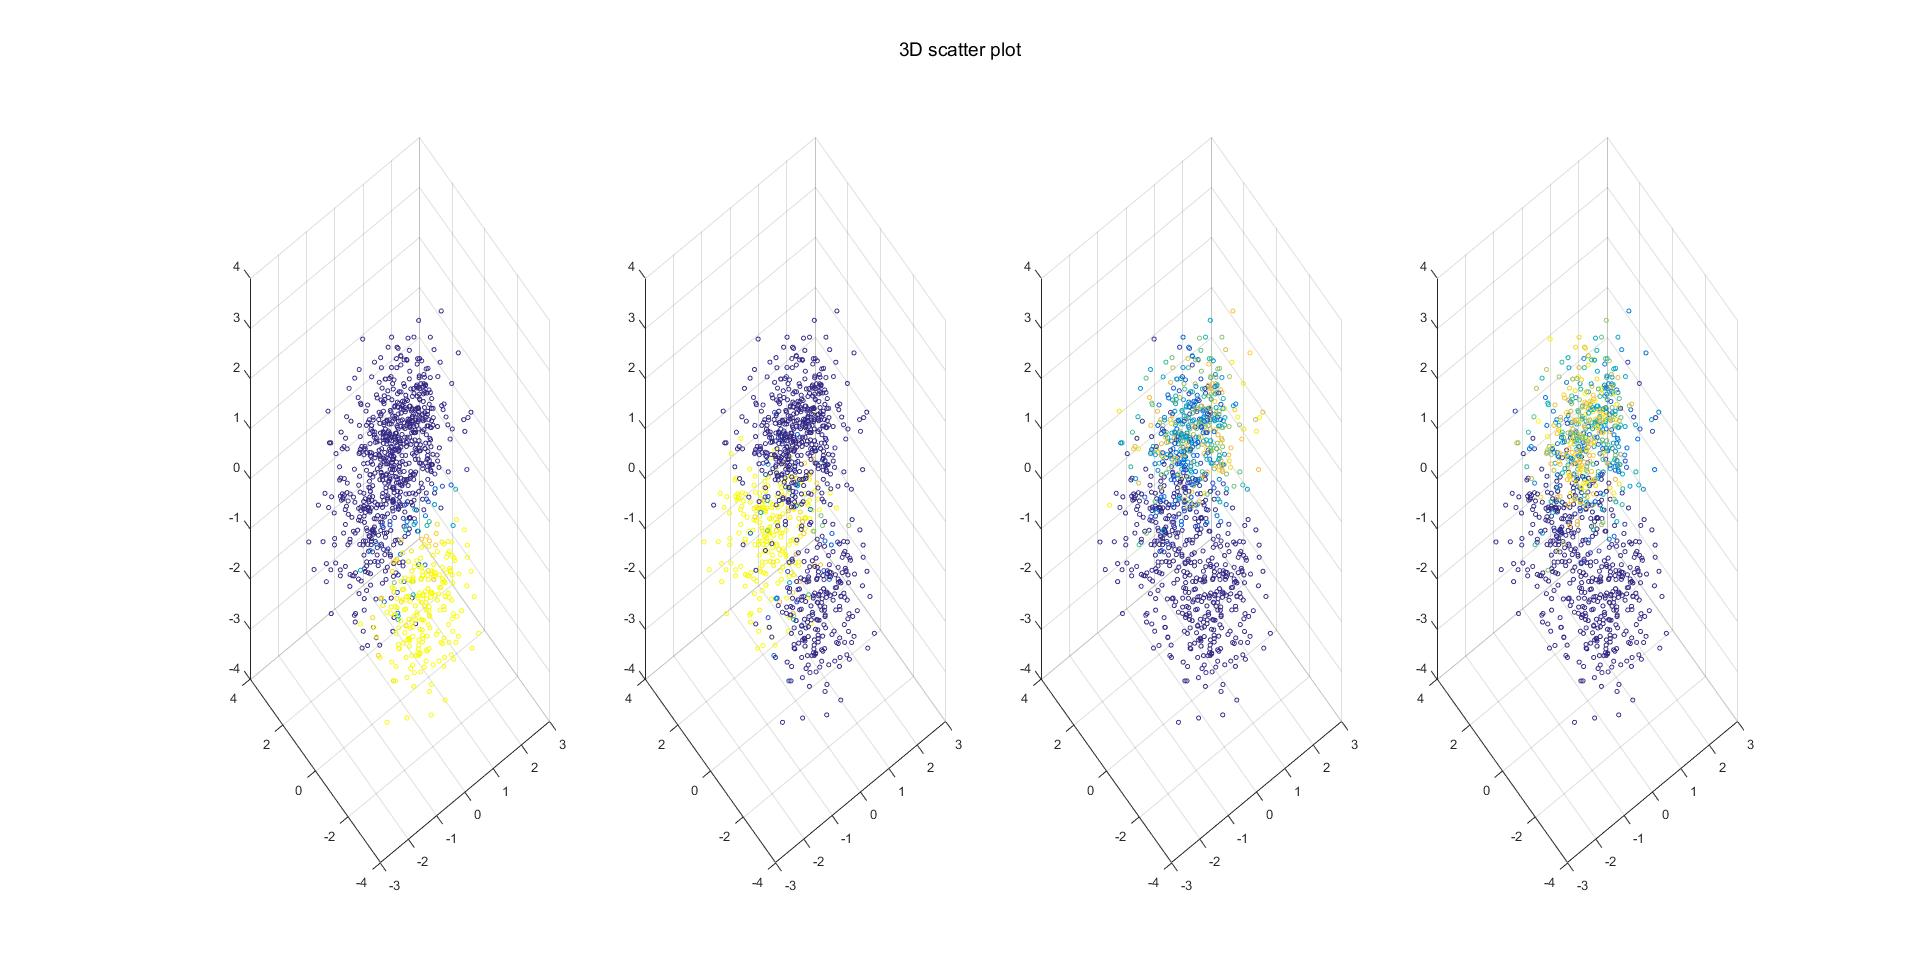
\includegraphics[width = 6in]{scatter3d4.jpg}
\caption{3-d scatter plot assuming 4 component}
\end{figure}


If assuming 5 mixture components, the mixture proportions as well as the mean and covariance for every cluster are not consistent. The results of experiments I did are shown below, the parameters learned are not consistent:
\begin{figure}[H]
\centering
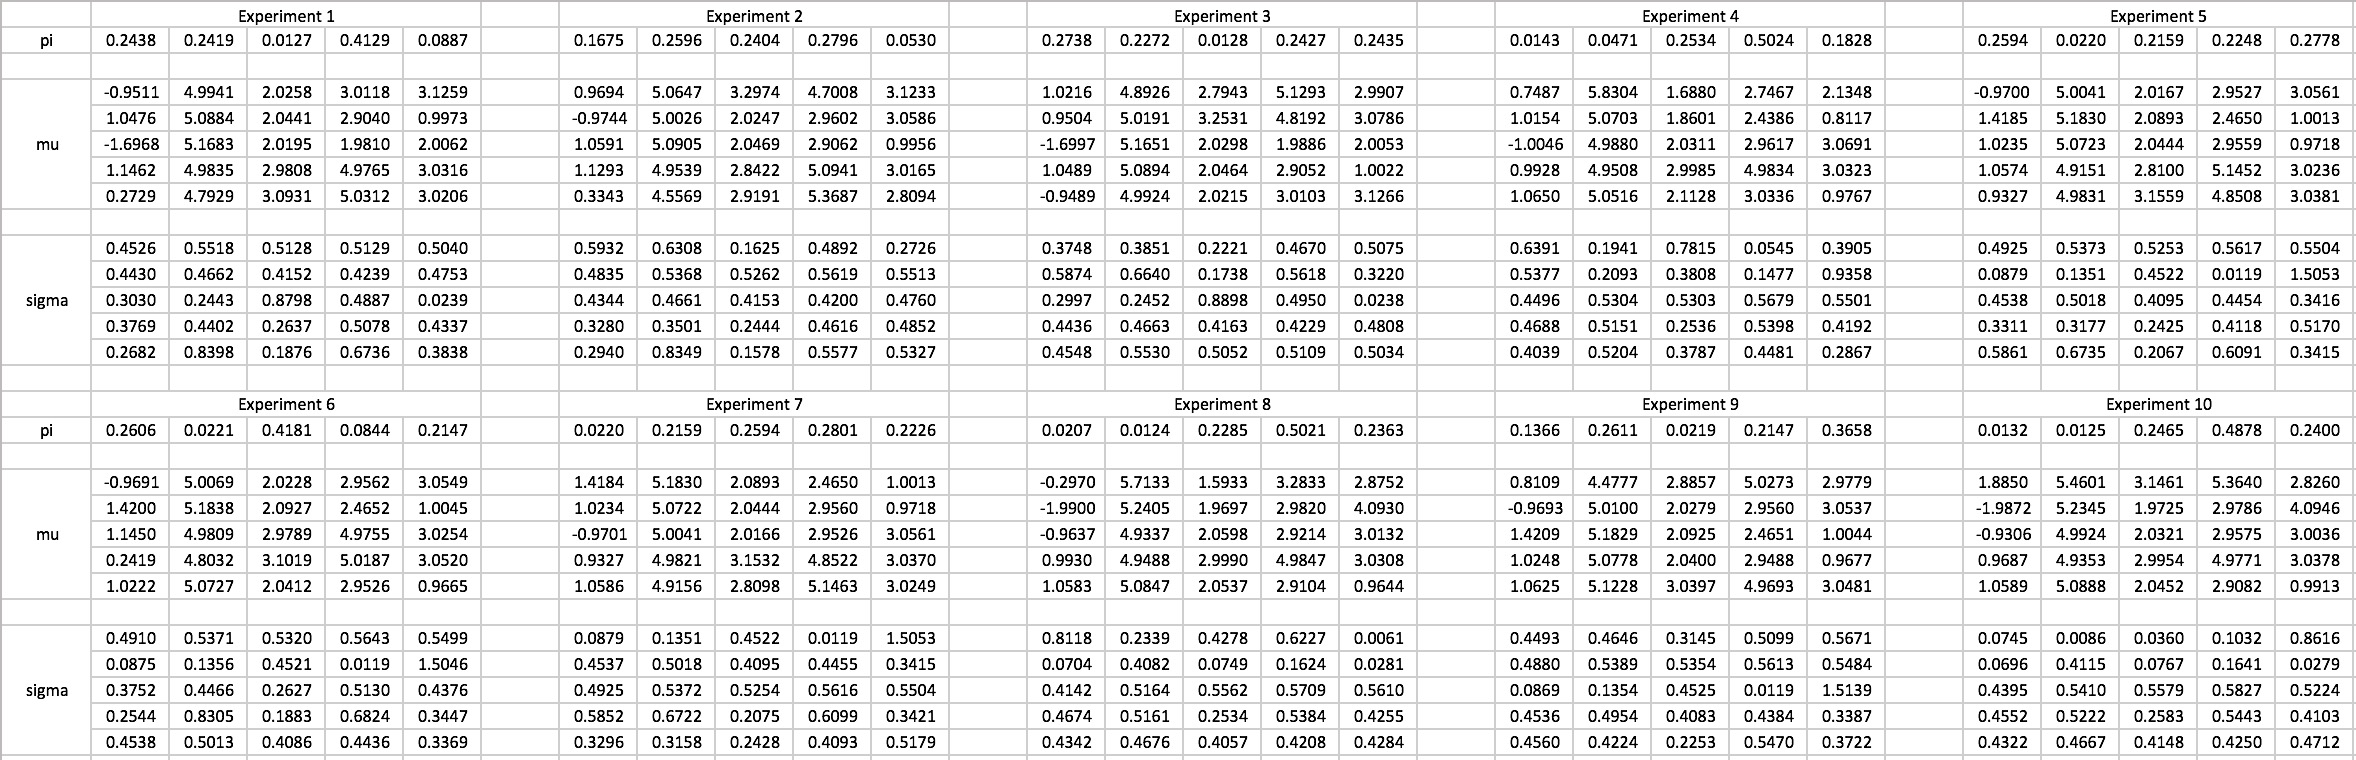
\includegraphics[width = 7in]{EM5.jpg}
\end{figure}
The proportion of one or two component(s) are tend to be small, which indicates merging with other components.\\
One of the scatter plots are shown below:
\begin{figure}[H]
\centering
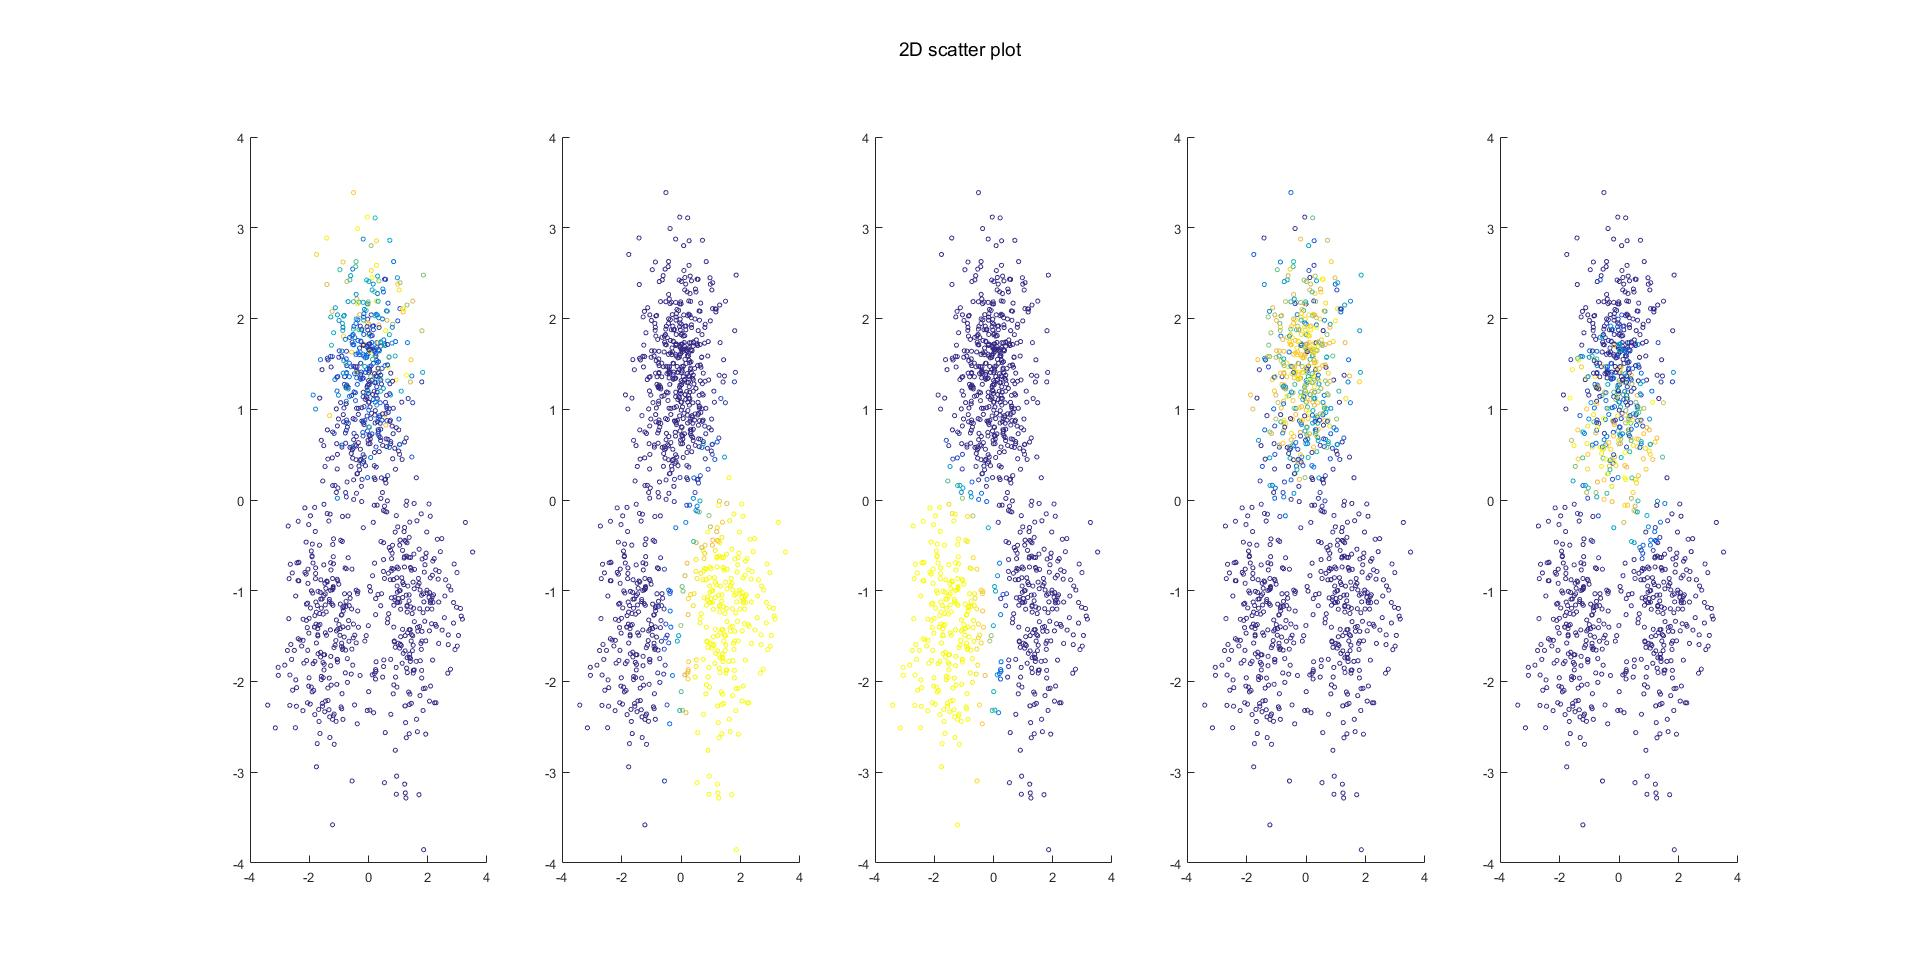
\includegraphics[width = 6in]{scatter2d5.jpg}
\end{figure}

\begin{figure}[H]
\centering
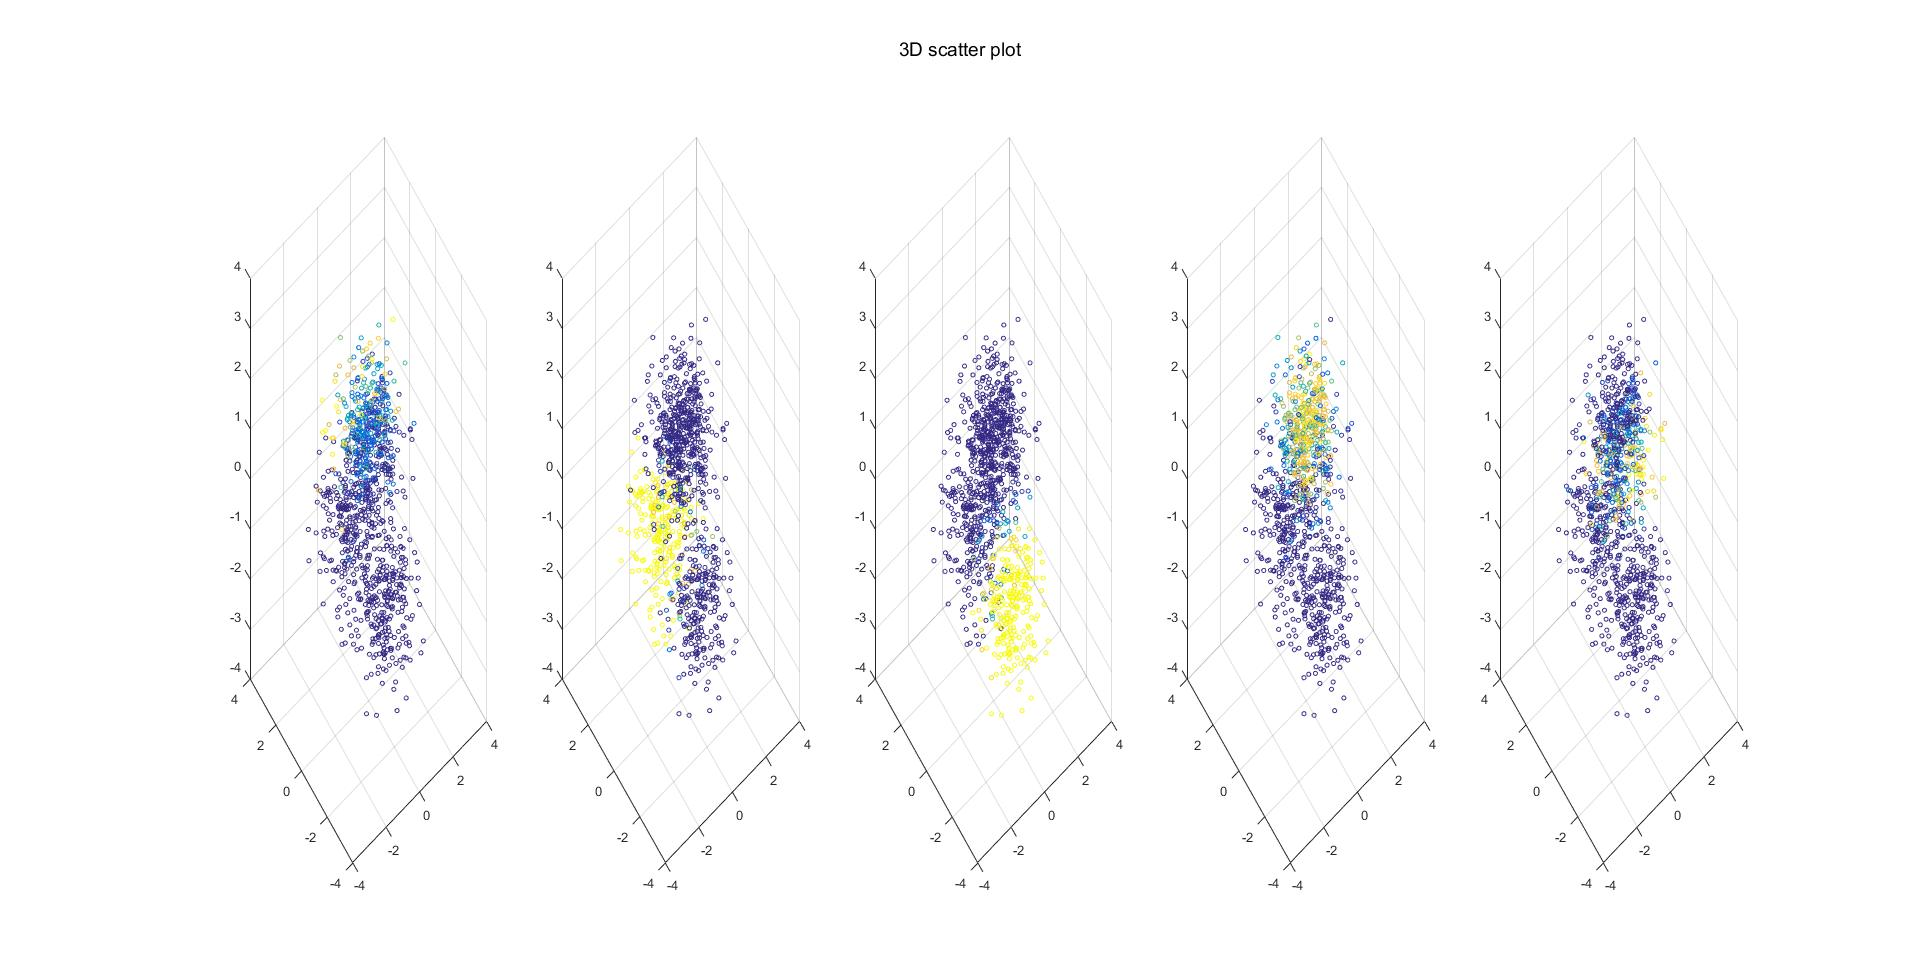
\includegraphics[width = 6in]{scatter3d5.jpg}
\end{figure}
From the figures we can also see that there are two clusters which are pretty consistent, but the other three are always mixing together. And by run the EM code several, the parameters changed a lot and are not consistent. \\

\item My estimate for the mixture proportions are $p_1 = 0.2397$, $p_2 = 0.5014$, $p_3 = 0.2589$.\\
My estimate for the means are:\\
 $\mu_1 = \begin{bmatrix} 1.0571 & 5.0886 & 2.0447 & 2.9064 & 0.9899\end{bmatrix}$, \\
 $\mu_2 = \begin{bmatrix} 0.9925 & 4.9494 & 3.0000 & 4.9870 & 3.0304\end{bmatrix}$, \\
 $\mu_3 = \begin{bmatrix} -0.9795 & 5.0040 & 2.0273 & 2.9582 & 3.0587\end{bmatrix}$ \\
 My estimate for the covariances are:\\
 $\Sigma_1 = \begin{bmatrix} 0.4340 & 0 & 0 & 0 & 0\\0 & 0.4662 & 0 & 0 & 0\\0 & 0 & 0.4143 & 0 & 0\\0 & 0 & 0 & 0.4238 & 0\\0 & 0 & 0 & 0 & 0.4690\end{bmatrix}$, \\
  $\Sigma_2 = \begin{bmatrix} 0.4678 & 0 & 0 & 0 & 0\\0 & 0.5159 & 0 & 0 & 0\\0 & 0 & 0.2524 & 0 & 0\\0 & 0 & 0 & 0.5360 & 0\\0 & 0 & 0 & 0 & 0.4245\end{bmatrix}$, \\
   $\Sigma_3 = \begin{bmatrix} 0.4782 & 0 & 0 & 0 & 0\\0 & 0.5377 & 0 & 0 & 0\\0 & 0 & 0.5336 & 0 & 0\\0 & 0 & 0 & 0.5612 & 0\\0 & 0 & 0 & 0 & 0.5520\end{bmatrix}$
\end{enumerate}

\newpage
\section*{\huge\textbf{ MATLAB code used in this report }  }
\Large{The \textbf{main script} for \textbf{Problem 1}}
\normalsize
\begin{lstlisting}
dbstop if error
close all
clear
clc
data1 = importdata('RedWine_HW7.txt');
redWine = data1.data;
data2 = importdata('WhiteWine_HW7.txt');
whiteWine = data2.data;
d0 = size(redWine,2); % get the original dimension of the data set
%% Preprocessing
redW = (redWine-min(redWine))./(max(redWine)-min(redWine)); % normalize the data
whiteW = (whiteWine-min(whiteWine))./(max(whiteWine)-min(whiteWine)); % normalize the data
% redW = redWine; % not normalize the data
% whiteW = whiteWine; % not normalize the data
N1 = size(redW,1);
N2 = size(whiteW,1);
%% Forward Feature Selection (FFS)
d_list = 1:d0;
d_seqFFS = [];
for ii = 1:d0
	for jj = 1:length(d_list)
        ratio_FFS(ii,jj) = calculateFisherRatio(redW(:,[d_seqFFS, d_list(jj)]), ...
        whiteW(:,[d_seqFFS, d_list(jj)]));
	end
	d_seqFFS(ii) = find(ratio_FFS(ii,:) == max(ratio_FFS(ii,:)));
end
for i = 1:d0
    temp(i) = ratio_FFS(i,d_seqFFS(i));
end
figure, plot(temp, 'Linewidth', 2), hold on, plot(temp, '.', 'Linewidth', 8)
grid on, xlabel('iteration'), ylabel('Fisher ratio'), title('Performance curve of FFS')
%% Backward Feature Selection (BFS)
d_list = 1:d0;
d_seqBFS = [];
for ii = 1:(d0-1)
    for jj = 1:length(d_list)
        idx_list = d_list;
        idx_list(jj) = [];
        ratio_BFS(ii,d_list(jj)) = calculateFisherRatio(redW(:,idx_list), ...
        whiteW(:,idx_list));
    end
    temp = ratio_BFS(ii,:);
    d_seqBFS(ii) = find(ratio_BFS(ii,:) == max(temp(temp>0)));
    d_list(d_list == d_seqBFS(ii)) = [];
end
for i = 1:(d0-1)
    temp(i) = ratio_BFS(i,d_seqBFS(i));
end
figure, plot(temp, 'Linewidth', 2), hold on, plot(temp, '.', 'Linewidth', 8)
grid on, xlabel('iteration'), ylabel('Fisher ratio'), title('Performance curve of BFS')
\end{lstlisting}


\Large{The function \textbf{``calculateFisherRatio"} used in the main script}
\normalsize
\begin{lstlisting}
function ratio = calculateFisherRatio(D1, D2 )
%The function to calculate the Fisher Ratio
%   Input:
%      D1: data from class 1
%      D2: data from class 2
%  lambda: parameter for diagonal loading
D = [D1;D2];
d = size(D,2);
mu0 = mean(D,1);
n1 = size(D1,1);
n2 = size(D2,1);
pi1 = n1/(n1+n2);
pi2 = n2/(n1+n2);
mu1 = mean(D1,1);
mu2 = mean(D2,1);
Sw = pi1*(D1-mu1)'*(D1-mu1)/n1 + pi2*(D2-mu2)'*(D2-mu2)/n2;
Sm = (D-mu0)'*(D-mu0)/(n1+n2);
Sb = pi1*(mu1-mu0)'*(mu1-mu0) + pi2*(mu2-mu0)'*(mu2-mu0);
ratio = trace(Sb*pinv(Sw));
end
\end{lstlisting}

\Large{The \textbf{main script} for \textbf{Problem 2}}
\normalsize
\begin{lstlisting}
dbstop if error
close all
clear
clc
% GMM = importdata('GMDataSet_HW7.txt');
% save('GMM.mat', 'GMM')
load('GMM.mat') %GMM
%% PCA 
projected_GMM = PCA( GMM, 3);
%% main part: EM-GMM
numCom = 3;
[ mu, sigma, pi, C ] = EM_GMM( GMM, numCom );
for i = 1:numCom
    figure(101), subplot(1,numCom, i)
    scatter3(projected_GMM(:,1), projected_GMM(:,2), projected_GMM(:,3), 10, C(:,i))
%     title(['Mean: ', num2str(mu(i,:))])
    figure(102), subplot(1,numCom, i)
    scatter(projected_GMM(:,2), projected_GMM(:,3), 10, C(:,i))
%     title(['Mean: ', num2str(mu(i,:))])
end
figure(101), suptitle('3D scatter plot'), saveas(gcf, 'scatter3d.jpg')
figure(102), suptitle('2D scatter plot'), saveas(gcf, 'scatter2d.jpg')
\end{lstlisting}
The function ``PCA" used is the same that I used in homework 2, coded on my own.

\Large{The function \textbf{EM\_GMM} for \textbf{Problem 2}}
\normalsize
\begin{lstlisting}
function [ mu, sigma, pi, C ] = EM_GMM( data, num_com )
%function of expectation maximization for Gaussian Mixture Model
%   Input:
%    data: input data
% num_com: number of components
%  Output:
%      mu: means learned by EM
%   sigma: variances learned by EM (only consider diagonal covariance matrix)
%      pi: probabilities of a data coming from a component

% initialization
maxIter = 600;
thres = 0.0001;
d = size(data,2); % dimension of data
N = size(data,1); % # of data points
for i = 1:num_com
    mu(i,:) = data(max(1,round(N*rand)),:);
    sigma(i,:) = ones(1,d);
    pi(i) = 1/num_com;
end
% E-step
for k = 1:num_com
    C(:,k) = mvnpdf(data, mu(k,:), sigma(i)*eye(d))*pi(k);
end
C = C./repmat(sum(C,2),[1,num_com]);
% M-step
diff = inf;
numIter = 1;
while (diff>thres && numIter <= maxIter)
    mu0 = mu;
    sigma0 = sigma;
    pi0 = pi;
    temp = sum(sum(C));
    for k = 1:num_com
        temp1 = sum(C(:,k),1); % sum_i(C_ik)
	% update mu
        mu(k,:) = sum(data.*repmat(C(:,k),[1,d]),1)/temp1;     
    % update sigma
    temp2 =  (data-repmat(mu(k,:), [N, 1]));
    J = zeros(size(sigma(k,:)));
    for i = 1:size(data,1)
        J = J+C(i,k)*temp2(i,:).^2;
    end
    sigma(k,:) = J/temp1;        
	%update pi
        pi(k) = temp1/temp;
    end    
    %update C_ik
    for k = 1:num_com
%         C(:,k) = mvnpdf(data, mu(k,:), sigma(:,:,k))*pi(k);
        C(:,k) = mvnpdf(data, mu(k,:), sigma(k,:)*eye(d))*pi(k);
    end
    C = C./repmat(sum(C,2),[1,num_com]);    
    diff = sum(sum(abs(mu0-mu))) + sum(sum(abs(sigma0-sigma))) + sum(abs(pi0-pi));
    numIter = numIter+1;
end
end
\end{lstlisting}
\end{spacing}
\end{document}